\documentclass{article}
\usepackage{ctex} % Include the ctex package to support Chinese
\usepackage{graphicx} % For inserting images
\usepackage{geometry} % For setting page layout
\usepackage{booktabs} % For beautifying tables
\usepackage{enumitem} % For customizing list formats
\usepackage{lipsum}  % Package for generating paragraphs
\usepackage{ctex} % Include the ctex package to support Chinese
\usepackage{graphicx} % Load the graphic handling package
\usepackage{booktabs} % For beautifying table lines
\usepackage{caption} % For adding table captions
\usepackage[table]{xcolor} % For setting table colors
\usepackage{float}
\usepackage{makecell}
\usepackage{subcaption}
\usepackage{tabularx}
\usepackage{tcolorbox}
\tcbuselibrary{listings}
\usepackage{array}
\usepackage[dvipsnames]{xcolor}
\usepackage{tikz}
\usepackage{hyperref} 
\usepackage{framed}
\usetikzlibrary{positioning} % Load the positioning library
\renewcommand{\refname}{}

\hypersetup{
    colorlinks=true, % Use colors instead of boxes
    linkcolor=black, % Link color is black
    citecolor=black, % Citation color is black
    urlcolor=blue    % URL color is blue (can be modified as needed)
}
\lstset{
 basicstyle=\ttfamily, % Set font family
 breaklines=true, % Automatic line wrapping
 keywordstyle=\bfseries\color{NavyBlue}, % Set keywords to bold, color is NavyBlue
 morekeywords={}, % Set more keywords, separated by commas
 emph={self}, % Specify emphasized words, separated by commas if multiple
    emphstyle=\bfseries\color{Rhodamine}, % Style for emphasized words
    commentstyle=\itshape\color{black!50!white}, % Set comment style, italic, light gray
    stringstyle=\bfseries\color{PineGreen!90!black}, % Set string style
    columns=flexible,
    % numbers=left, % Display line numbers on the left
    % numbersep=2em, % Set the position of line numbers
    % numberstyle=\footnotesize, % Shrink line numbers
    % frame=single, % Border
    framesep=1em, % Set the distance between code and border
	tabsize=2, % Set tab width to 2 spaces
    showstringspaces=false, % Do not show spaces in strings
}

\geometry{a4paper, margin=1in}
\begin{document}

\begin{titlepage}
    \centering
    \vspace*{1cm}

    % Insert school logo
    
\includegraphics[width=\textwidth]{img/logo.png} % Assume logo.png is the school logo image file

    % \vspace{1.5cm}
    \fontsize{24pt}{32pt}\selectfont
    \textbf{《High-level Language Programming Project》 Report}
    \vspace{4cm}

    \centering
    Ztest: A C++ Unit Testing Framework
    \vspace{2cm}

    \fontsize{16pt}{16pt}\selectfont
    \begin{tabular}{ll}                                                                \\
        School       :   & School of Future Technology\hspace{6cm}          \\
        Major        :   & Data Science and Big Data Technology\hspace{6cm} \\
        Student Name :   & Zheng Chenyang,Ye Suohua,Wu Hongqing,            \\
                         & Qi Yansong,Wang Ruizhen                          \\
        Teacher      :   & Zhang Huaidong\hspace{6cm}                       \\
        Submission Date: & 2025.6.6\hspace{6cm}                             \\
    \end{tabular}

    \vfill

    \vspace{1cm}
\end{titlepage}

\tableofcontents  % Generate table of contents
\newpage
\section{Abstract}
Ztest is an innovative C++ unit testing framework designed to address limitations in existing tools like Google Test, such as lack of GUI support, poor concurrency handling, and inadequate reporting systems. It introduces a layered architecture combining object-oriented design, functional programming, and metaprogramming, with core modules including a test executor, data-driven testing system, and AI-powered diagnostics. Key features include:
\begin{enumerate}
    \item \textbf{Parallel Execution}: Safe tests are run concurrently via a thread pool (8-thread default), reducing execution time compared to sequential frameworks.
    \item \textbf{Data-Driven Testing}: Implements parameterized tests with CSV integration and LRU caching, accelerating large-scale test execution.
    \item \textbf{Smart Diagnostics}: Integrates Qwen Turbo API for failure root cause analysis, test coverage assessment, and stability recommendations in HTML reports.
    \item \textbf{Cross-Platform GUI}: Built with ImGui and MVC architecture, supporting real-time resource monitoring, test filtering, and AI-assisted debugging.
    \item \textbf{Extensible Reports}: Generates HTML/XML/JSON reports compatible with CI/CD pipelines, including detailed benchmark metrics and visualizations.
\end{enumerate}
\section{System Requirements Analysis}

\subsection{System Background and Motivation}
% Fill in the content of system background and motivation here
With the increasing demand for complex system architecture design capabilities, mastering object-oriented design principles and pattern-based engineering practices has become a core goal of advanced software engineering education. This not only requires an understanding of the dynamic collaboration between classes and objects, but also the ability to solve architectural challenges through design patterns with abstract thinking skills.
Existing unit testing frameworks (such as Google Test) have several drawbacks, including a steep learning curve, limited concurrency support, overly simplistic reporting systems, and average extensibility. Our team plans to develop a flexible, efficient, and easy-to-use testing tool (with a graphical user interface, GUI) to provide an intuitive and user-friendly environment for developers and testers to write, run, and manage test cases. This tool will support various types of tests (such as unit tests and integration tests) and provide detailed test result reports.
\begin{table}[h]
    \centering
    \caption{Comparison of Mainstream Testing Frameworks}
    \label{tab:compare}
    \begin{tabularx}{\textwidth}{lXXXX}
        \toprule
        \textbf{Framework}       & \textbf{GUI Support} & \textbf{Concurrent Testing} & \textbf{Report System} & \textbf{Data-Driven} \\
        \midrule
        Google Test (C++)        & Third-Party          & Limited                     & Basic                  & Not Supported        \\
        JUnit    (Java)          & Eclipse Plugin       & Supported                   & HTML/XML               & Supported            \\
        PyTest (Python)          & Third-Party          & Excellent                   & Rich                   & Supported            \\
        Catch2   (C++)           & None                 & Average                     & Concise                & Not Supported        \\
        % \midrule
        \textbf{Ztest*}    (C++) & Excellent            & Excellent                   & Rich                   & Supported            \\
        \bottomrule
    \end{tabularx}
\end{table}
\subsection{System Objectives}
\begin{figure}[H]
    \centering
    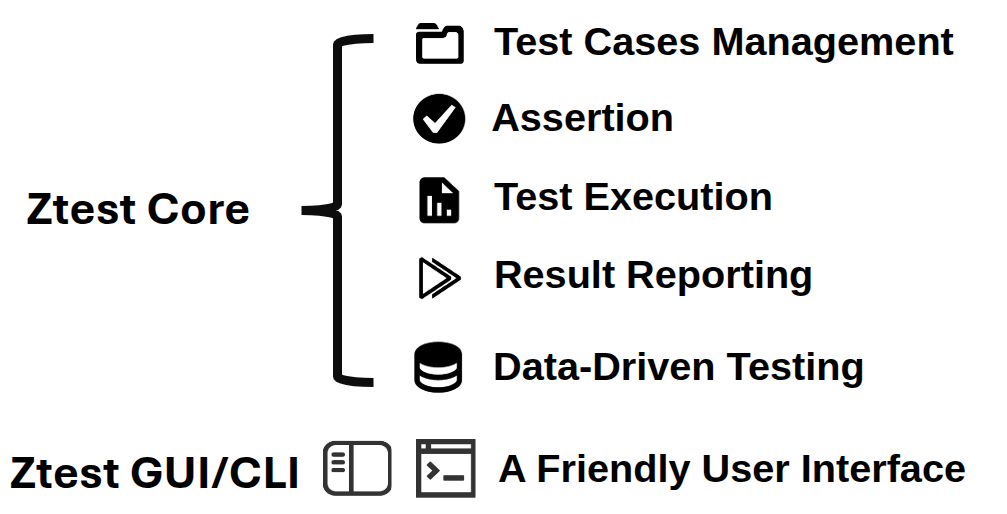
\includegraphics[width=0.6\textwidth]{img/func.png} % Assume logo.png is the school logo image file
    \caption{Ztest Function}
    \label{fig:ztest function }
\end{figure}
\subsubsection{Test Management}
% We categorize tasks into four types: short test time and more focused on result correctness, such as addition operations, string concatenation, and user login verification; long test time and more focused on result correctness, such as merging multiple files, complex string matching and replacement, and large data sorting result verification; short test time and more focused on process evaluation, such as reading or writing large files, low-complexity algorithm performance testing, and database queries; and long test time and more focused on process evaluation, such as multi-threaded processing tasks, stress testing, and high-time-complexity algorithm testing.

% \begin{figure}[H]
%     \centering
%     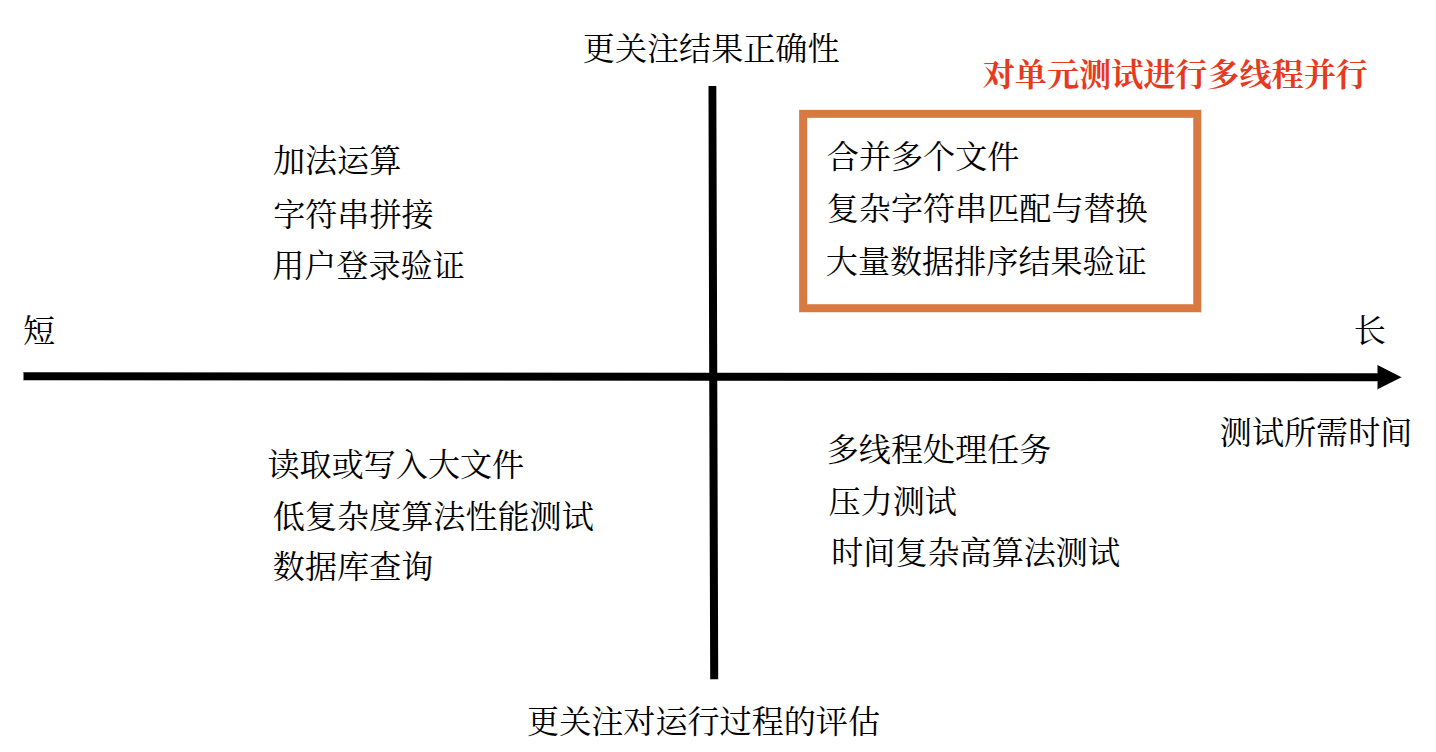
\includegraphics[width=0.6\textwidth]{img/task.png} % Assume logo.png is the school logo image file
%     \caption{Task Type}
%     \label{fig:ztest task type }
% \end{figure}

Compared to traditional unit testing frameworks, Ztest supports various test types, such as parallel and thread-safe tests, serial or thread-unsafe tests, performance evaluation through iteration, and parameterized data-driven tests. We provide test fixtures to manage individual tests.

\begin{figure}[H]
    \centering
    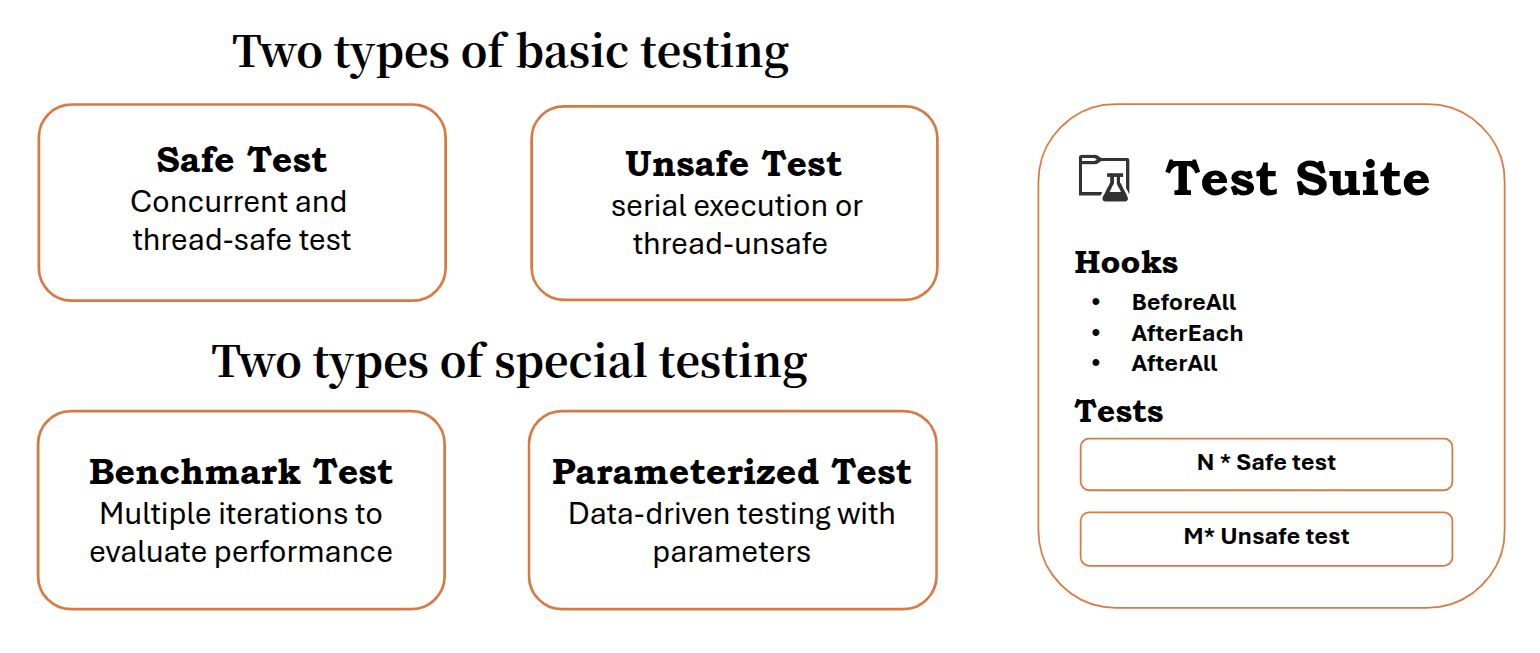
\includegraphics[width=0.8\textwidth]{img/types.png} % Assume logo.png is the school logo image file
    \caption{Test Types}
    \label{fig:test types }
\end{figure}
We provide macros similar to Google Test to simplify test definition:
\begin{framed}
    \begin{lstlisting}[language=C++]
ZTEST_F(SuiteName, TestName, safe/unsafe) { ... } // Define a test 
ZBENCHMARK(SuiteName, TestName, iterations) { ... } // Define a benchmark
ZTEST_P(SuiteName, TestName, data) { ... }  // Define a parameterized test
ZTEST_P_CSV(SuiteName, TestName, "data.csv") { ... } // Define a parameterized test with csv data
\end{lstlisting}
\end{framed}

At the same time, we can chain test case definitions:
\begin{framed}
    \begin{lstlisting}[language=C++]
auto test_case = TestFactory::createTest("Add", ZType::Z_SAFE, "", add, 2, 3)
                 .setExpectedOutput(5)
                 .beforeAll([]() { logger.info("Init\n"); })          
                 .afterEach([]() { logger.info("Clean\n"); }).build();
                \end{lstlisting}
\end{framed}

\subsubsection{Assertion Mechanism}
The assertion mechanism is used to verify whether the expected results of test cases are correct. The framework provides a variety of assertion macros, such as \textbf{EXPECT\_EQ} and \textbf{ASSERT\_TRUE}, to quickly verify conditions in tests.
The main assertions provided are:
\begin{itemize}
    \item \textbf{EXPECT\_EQ}: Verifies whether two values are equal.
    \item \textbf{ASSERT\_TRUE}: Verifies whether a condition is true.
    \item \textbf{EXPECT\_NEAR}: Verifies whether two floating-point values are close enough.
\end{itemize}
Usage example:
\begin{framed}

    \begin{lstlisting}[language=C++]
// If the assertion fails, an exception is thrown
EXPECT_EQ(5, add(2, 3));
ASSERT_TRUE(6 == add(2, 3));
EXPECT_NEAR(5.0, add(2.0, 3.0), 0.1);
\end{lstlisting}
\end{framed}

If an assertion fails, a \textbf{ZTestFailureException} exception is thrown. You can also inherit from the \textbf{ZTestFailureException} to customize the exception handling logic.
\subsubsection{Data-Driven Testing}
Parameterized testing refers to replacing certain fixed data in test cases with parameters during the testing process, and then generating multiple sets of test data by changing the values of the parameters to perform multiple tests on the software. It allows testers to cover multiple input scenarios with a single set of test logic, instead of writing separate test code for each scenario.
A data-driven testing framework (Data-Driven Testing Framework) is an automated testing framework that separates test data from test scripts and drives test case execution through external data sources (such as Excel, CSV files, databases, etc.).

ZTest implements parameterized testing and data-driven testing by importing and parsing data from CSV files. To accelerate data access, the imported data is cached. A lazy loading mechanism is used, where data is only loaded into the cache when needed, reducing unnecessary resource consumption. At the same time, an LRU cache eviction strategy is used to ensure that the data in the cache is the most likely to be accessed again, thereby maximizing the effectiveness of the cache.

\subsubsection{Test Executor}
The test executor is responsible for managing the execution of test cases, supporting \textbf{concurrent} execution of test cases and collecting test results, implementing automatic scheduling of tests and test result statistics.
Its behavior is as follows:
\begin{itemize}
    \item Concurrently run safe tests. Thread creation and destruction are relatively time-consuming operations. Using a thread pool to manage the lifecycle of threads allows for thread reuse, avoiding frequent thread creation and destruction, thereby significantly improving system performance.
    \item Serially run unsafe tests. A queue is used to maintain the order of test cases to ensure sequential execution.
    \item Serially run Benchmark tests.
    \item Serially run Parameterized tests.
\end{itemize}
\subsubsection{Report Generation}
It can generate HTML, JSON, and XML reports for convenient viewing of test results and integration with CI/CD.
\begin{figure}[H]
    \centering
    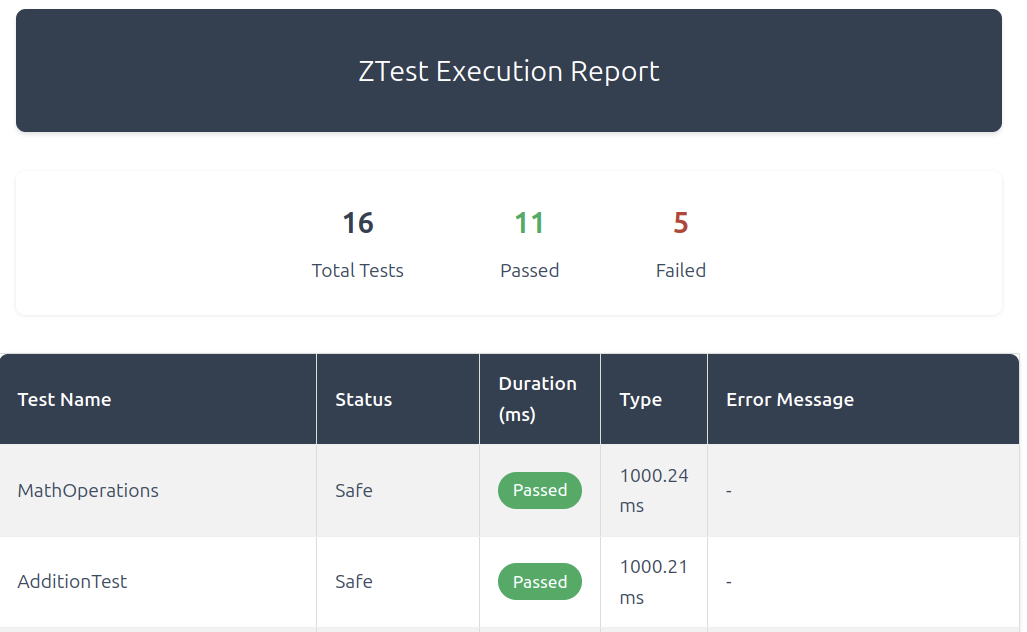
\includegraphics[width=0.8\textwidth]{img/report.png}
    \caption{Test Result Display Interface Layout}
    \label{fig:report}
    \small
\end{figure}
\subsubsection{CLI Interface}
\begin{framed}
    \begin{lstlisting}
Usage: executor_name [OPTIONS] 
Options: 
--help                         Show help 
--run-all                      Run all tests
--list-tests                   List all tests
--no-gui                       Run in headless mode
\end{lstlisting}
\end{framed}

\subsubsection{GUI Display}
The GUI can display test results, filter test results, monitor system resource status, and view details of a specific test run.
\begin{figure}[H]
    \centering
    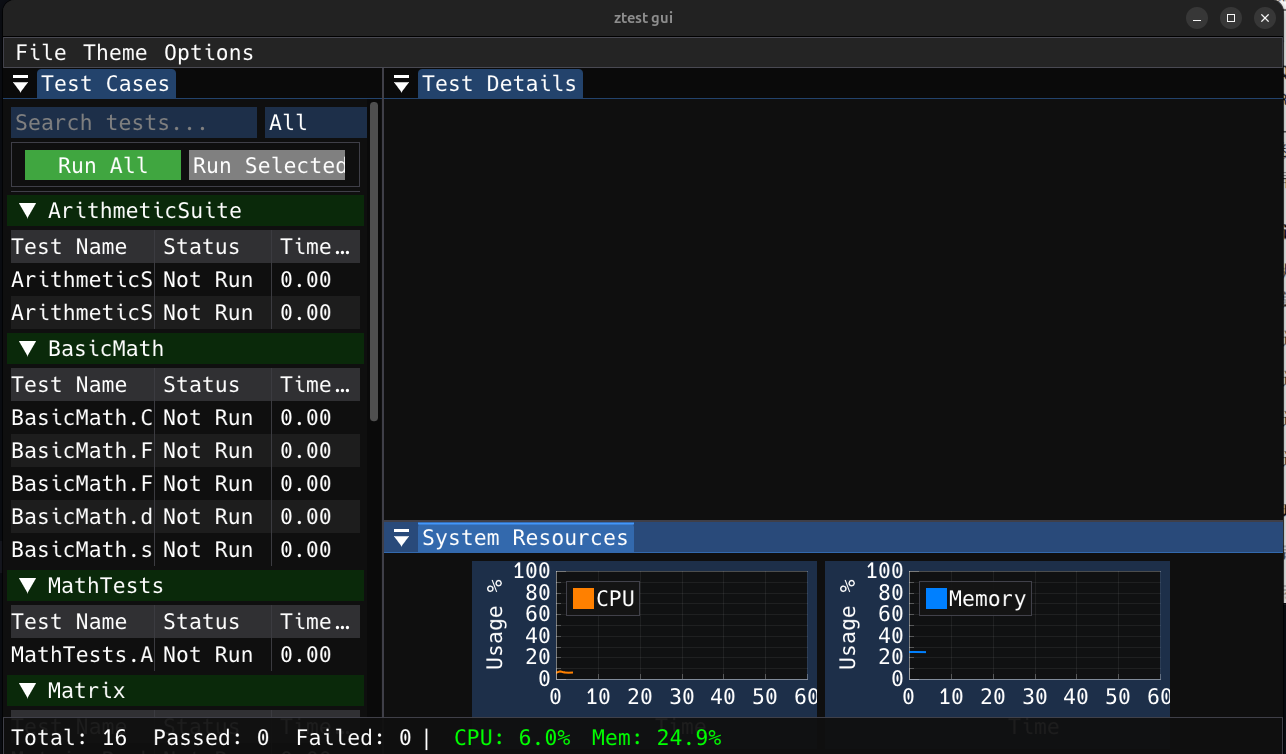
\includegraphics[width=\textwidth]{img/gui.png}
    \caption{Test Management Interface Layout}
    \label{fig:gui}
    \small
\end{figure}
\subsubsection{AI Intelligent Diagnosis Function}
By calling the qwen3 interface, an intelligent diagnosis function is realized. The report can include:
\begin{enumerate}
    \item Identifying the root cause of failures
    \item Providing repair suggestions
    \item Identifying high-risk test cases
    \item Assessing overall test coverage
    \item Offering suggestions for improving system stability
\end{enumerate}

You can also obtain specific analysis for a particular test case on the GUI interface, customize prompts, and upload source files to assist with analysis.
\newpage
\section{Program Analysis}
\subsection{Key System Issues}
\subsubsection{Excellent Architectural Design}
Ztest uses a layered architecture for the core modules, specifically as follows:
\begin{itemize}
    \item Basic Layer: Provides basic functions of the test framework, such as test case registration, test execution, test result management, and log output.
    \item Execution Layer: Manages the execution of test cases, including registration, execution, result management, and log output.
    \item Data Layer: Implements data-driven parameterized testing and provides data sources for test cases.
    \item Report Layer: Offers multi-format report output, such as HTML, JSON, XML, etc.
    \item Concurrency Layer: Encapsulates thread pool management for concurrent execution, improving testing efficiency.
\end{itemize}
\subsubsection{Application of Programming Design Ideas}
In the implementation process, Ztest uses five programming paradigms: object-oriented programming, generic programming, functional programming, concurrent programming, and metaprogramming.

\subsubsection{Improving Test Execution Efficiency}
Traditional C++ testing frameworks (such as gtest, catch2) mostly use sequential test execution methods, resulting in longer test times and reduced production efficiency. Meanwhile, the emergence of vibe coding has significantly reduced the time required to write test cases, but the time required to run test cases has not been significantly reduced.
We categorize tasks into four types: short test time and more focused on result correctness, such as addition operations, string concatenation, and user login verification; long test time and more focused on result correctness, such as merging multiple files, complex string matching and replacement, and large data sorting result verification; short test time and more focused on process evaluation, such as reading or writing large files, low-complexity algorithm performance testing, and database queries; and long test time and more focused on process evaluation, such as multi-threaded processing tasks, stress testing, and high-time-complexity algorithm testing.
\begin{figure}[H]
    \centering
    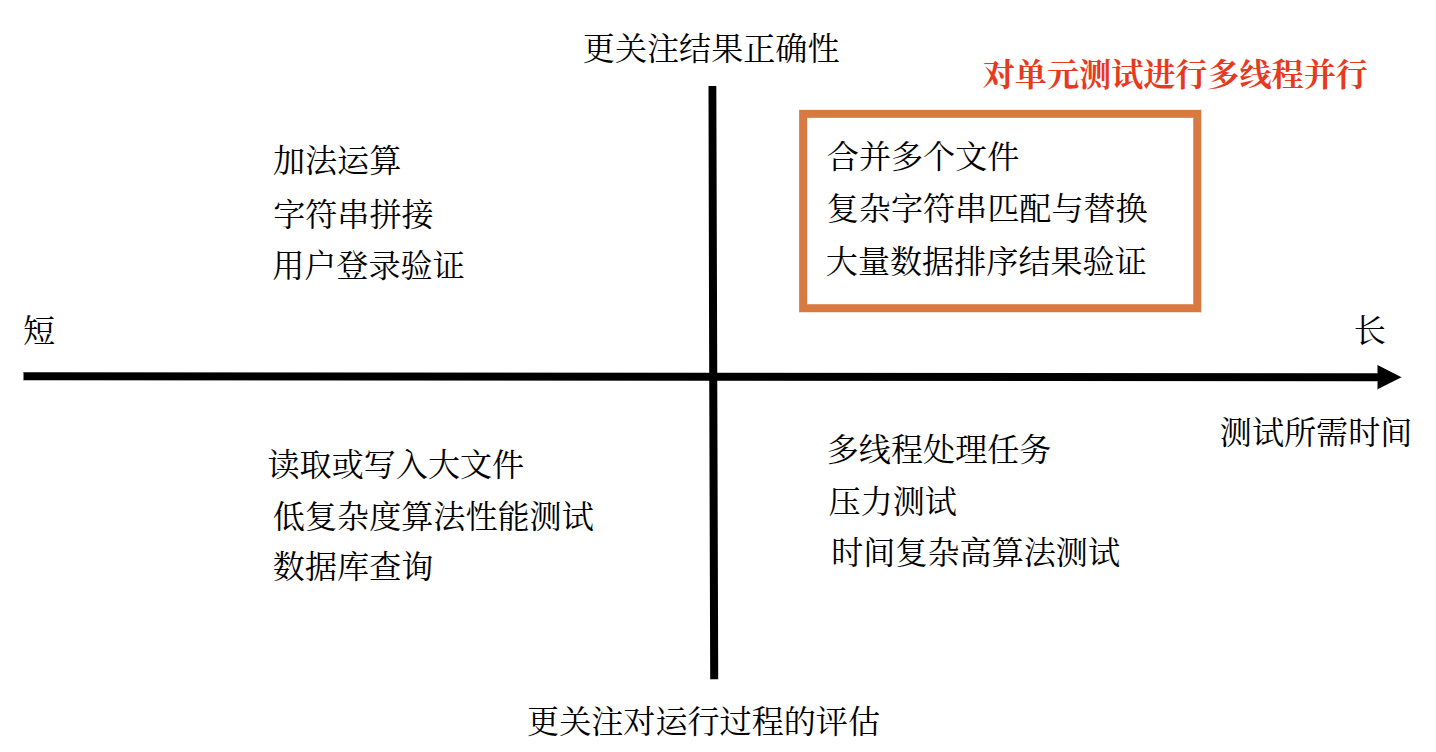
\includegraphics[width=0.8\textwidth]{img/task.png} % Assume logo.png is the school logo image file
    \caption{Task Types}
    \label{fig:task types }
\end{figure}
For tasks that take a long time to test, are more focused on result correctness, and are thread-safe, ZTest introduces concurrent test execution into the C++ testing framework system, directly integrating it into the test framework instead of using third-party tools like google-parallel, achieving finer-grained control.
At the same time, introducing data-driven testing and using caching to accelerate the definition and execution speed of large-scale unit tests is of great significance.
\subsubsection{Implementation of Syntactic Sugar}
How to encourage developers to use unit testing frameworks? The key lies in the simplicity of syntax definition. We use a series of complex macro definitions to implement syntactic sugar, thereby simplifying user definitions.
\subsubsection{Automatic Type Inference for Functions to Be Tested}
When defining a single test case in a chained manner, we hope that users only need to provide the function name, parameters, and expected results, and our framework will take over the specific logic of running and comparing test results. This requires us to automatically infer the parameter types of the function to be tested so that the function can be called for testing and test result verification. We use the factory pattern to specify the return type and the builder pattern to construct parameters and set expected results.
\subsection{Responsibilities Allocation}
% Fill in the responsibilities allocation for each student here
\begin{itemize}[leftmargin=*]
    \item Zheng Chenyang: Architectural design, main code writing for ztest core and GUI, report writing, and presentation
    \item Ye Suohua: GUI improvement, partial test logic improvement
    \item Wu Hongqing: GUI improvement
    \item Qi Yansong: GUI improvement
    \item Wang Ruizhen: Attempt to migrate to Windows
\end{itemize}

\section{Technical Approach}
\subsection{Operating Environment}
\begin{table}[H]
    \centering
    \caption{Development and Operating Environment}
    \begin{tabular}{@{}>{\bfseries}c>{\raggedright\arraybackslash}p{10cm}@{}} % Set the first column to bold and the second column to left-aligned
        \toprule
        \textbf{Component}      & \textbf{Tool Used for Development}                    \\
        \midrule
        Processor               & Intel i9-14900HX (32) @ 5.800GHz                      \\
        Operating System        & Ubuntu 24.04.2 LTS x86\_64 (kernel 6.11.0-26-generic) \\
        Compiler                & gcc 13.3.0 or clang 18.1.3 (MSVC is not allowed)      \\
        Graphics API            & glfw 3.4 + glad 4.0.1                                 \\
        GUI Framework           & ImGui-1.91.7-docking                                  \\
        Data Visualization Tool & implot v0.16                                          \\
        Build System            & XMake v2.9.9+HEAD.40815a0                             \\
        C++ Standard            & C++20 (required)                                      \\
        \bottomrule
    \end{tabular}
\end{table}
\subsection{Overall Design}
\subsubsection{Ztest Core Architecture Diagram}
% Describe the overall design of the system here
\begin{figure}[H]
    \centering
    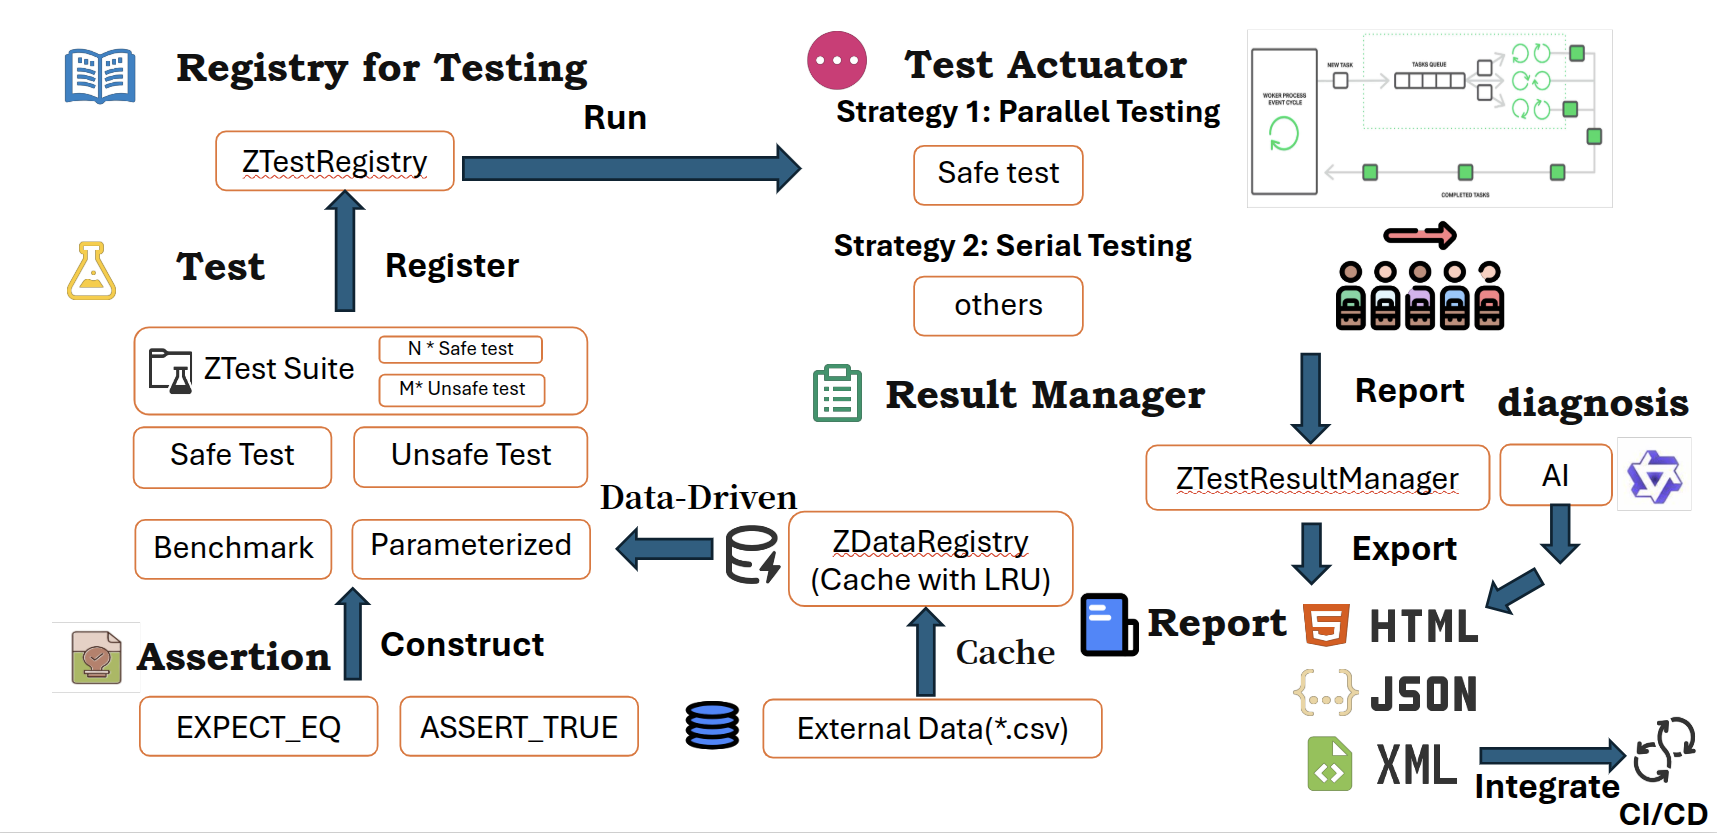
\includegraphics[width=\textwidth]{img/core.png} % Assume logo.png is the school logo image file
    \caption{Ztest Design}
    \label{fig:ztest design }
\end{figure}
The core architecture process of ZTest begins with the test definition stage, where tests (including ZTest Suite, safe tests, unsafe tests, benchmark tests, and parameterized tests) are defined using assertions such as EXPECT\_EQ and ASSERT\_TRUE to verify the correctness of test results.
Next, the tests are registered with the ZTestRegistry for unified management.
After registration, the tests are sent to the test executor, which adopts different test strategies based on the type of test. For safe tests, a parallel testing strategy is used, while other types of tests are executed serially.
During the execution of data-driven tests, the data-driven module manages external data (such as CSV files) through ZDataRegistry (with an LRU mechanism cache) to support test execution.
After testing is completed, the result manager ZTestResultManager is responsible for collecting and processing test results and exporting them in HTML, JSON, or XML formats for reporting and further analysis.
When exporting in HTML format, AI (qwen turbo) is used for test diagnosis and integrated into the HTML test report.
In addition, the entire testing process supports integration with Continuous Integration/Continuous Deployment (CI/CD) systems, allowing test results to be automatically fed back into the development process to improve software development efficiency and quality.
\begin{figure}[H]
    \centering
    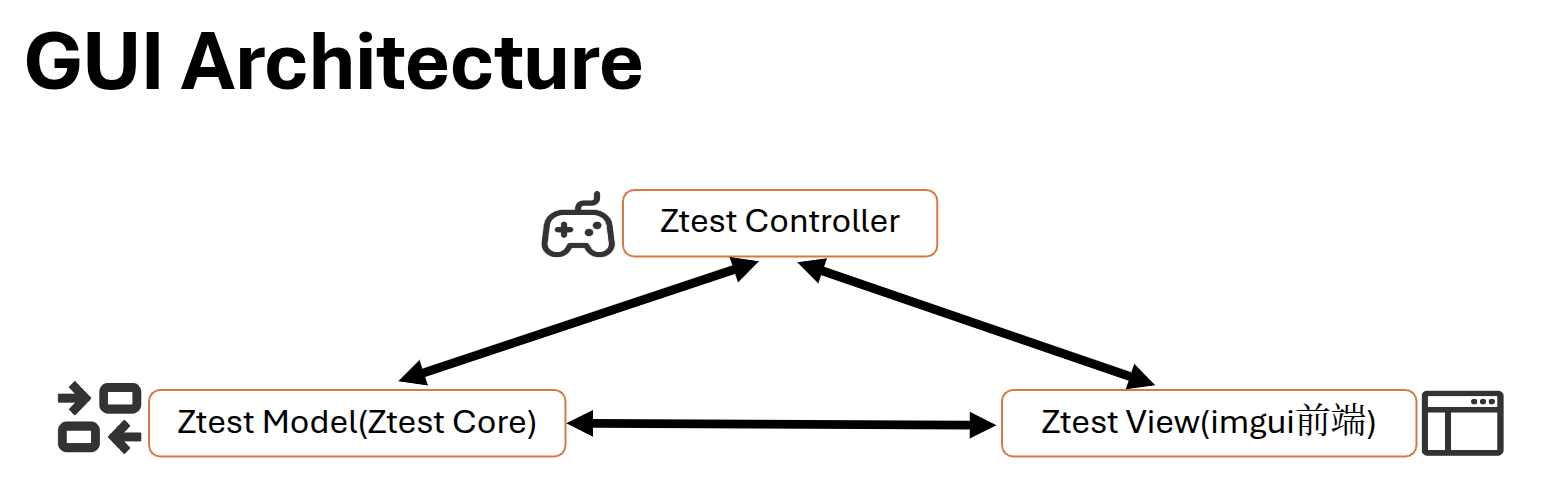
\includegraphics[width=0.8\textwidth]{img/guiarch.png} % Assume logo.png is the school logo image file
    \caption{Ztest GUI Architecture}
    \label{fig:ztest gui architecture }
\end{figure}
\subsubsection{GUI Framework}
The GUI framework is developed using the MVC architecture, where the Model layer is responsible for data processing (further encapsulating Ztest core), the View layer is responsible for interface drawing (mainly using the ImGui framework), and the Controller layer is responsible for user interaction, converting user operations on the UI interface (such as clicks and filtering) into calls to the Model and View layers to update the user interface and data.
\subsubsection{Overall Class Diagram}
\begin{figure}[H]
    \centering
    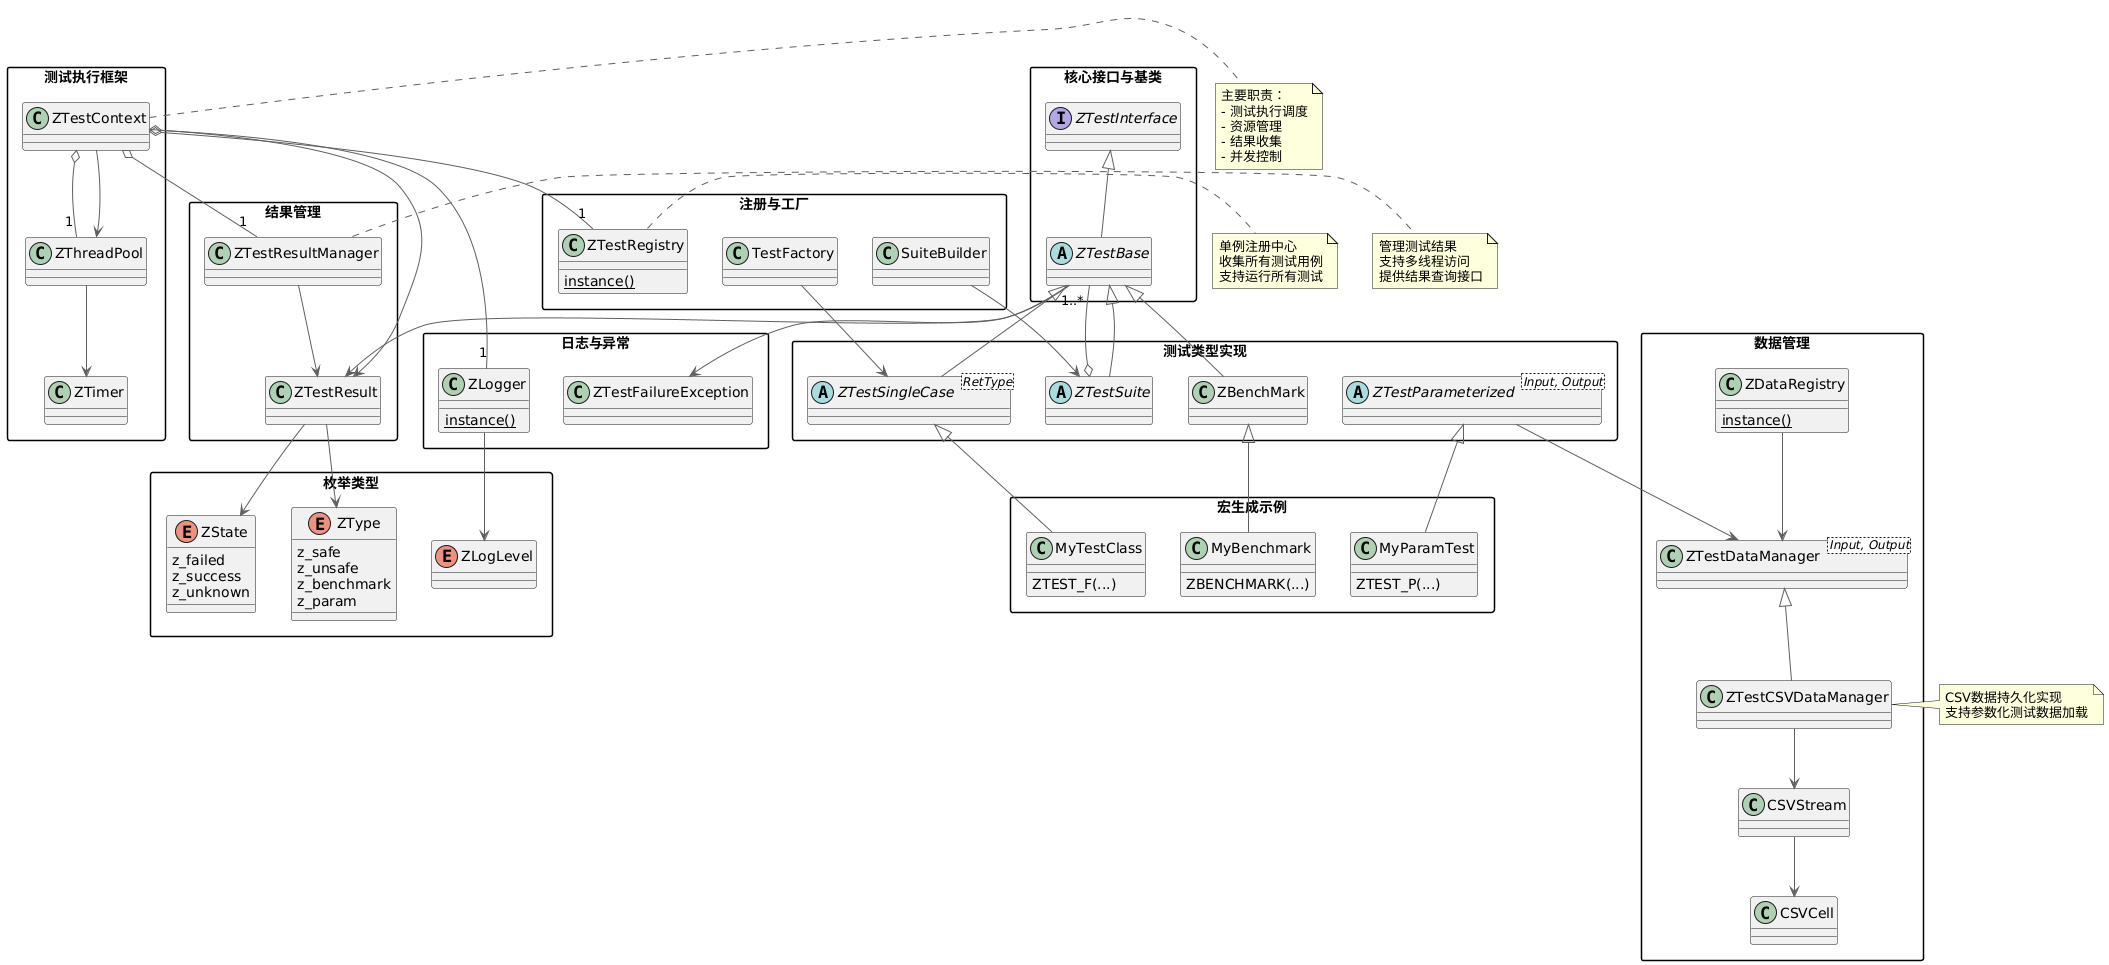
\includegraphics[angle=270,width=0.6\textwidth]{img/class.png} % Assume logo.png is the school logo image file
    \caption{Ztest Class Diagram}
    \label{fig:ztest class }
\end{figure}
\subsection{Detailed Design}
\subsubsection{Test Definition Related Classes}
\begin{itemize}
    \item \texttt{ZTestInterface}: The test interface defines the test execution framework.
    \item \texttt{ZTestBase} (ztest\_base.hpp): An abstract test base class that encapsulates common attributes and lifecycle hooks. It uses the Template Method pattern to define the test execution framework, implements the Strategy pattern through a virtual function table, and extends using hook functions with the Decorator pattern.
    \item \texttt{ZTestSingleCase} (ztest\_singlecase.hpp): A single test case implementation that uses the Template Method pattern to execute test logic, cooperates with TestFactory to demonstrate the Factory pattern, and supports chain configuration with the Builder pattern characteristics.
    \item \texttt{ZTestSuite} (ztest\_suite.hpp): A test suite class that inherits from ZTestBase, used to organize test cases, implements the Template Method pattern, and supports extension with hook functions.
    \item \texttt{ZBenchMark} (ztest\_benchmark.hpp): A benchmark test class that inherits from ZTestBase and overrides the run() method to implement benchmark testing through iterative execution of the test function.
    \item \texttt{ZTestParameterized} (ztest\_parameterized.hpp): A parameterized test base class that uses the Composite pattern to encapsulate test data and implements the data-driven testing framework through the run() method.
    \item \texttt{Macro Definition System} (ztest\_macros.hpp): Implements syntactic sugar through macro definitions, uses the Factory pattern to automatically generate test classes, and implements automatic registration with naming connection technology.
\end{itemize}
\begin{figure}[H]
    \centering
    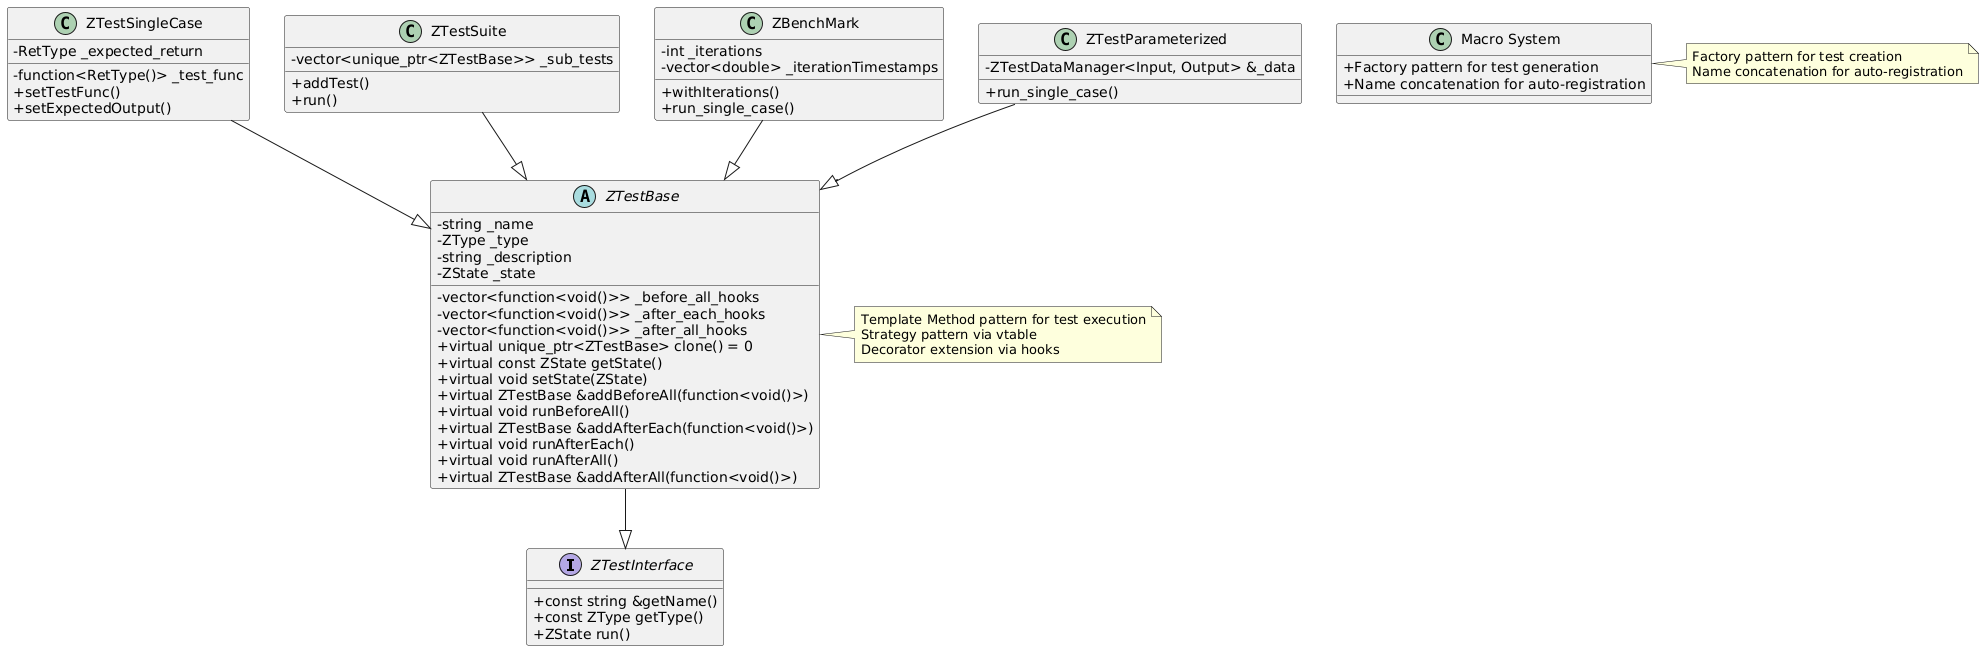
\includegraphics[width = \textwidth]{img/c1.png} % Assume logo.png is the school logo image file
    \caption{Ztest Class Diagram}
    \label{fig:ztest class }
\end{figure}

\subsubsection{Test Registration Related Classes}
\begin{itemize}
    \item \texttt{ZTestRegistry} (ztest\_registry.hpp): A global registration center implemented with the Singleton pattern, managing test case sets and ensuring thread-safe registration and retrieval operations.
\end{itemize}
\begin{figure}[H]
    \centering
    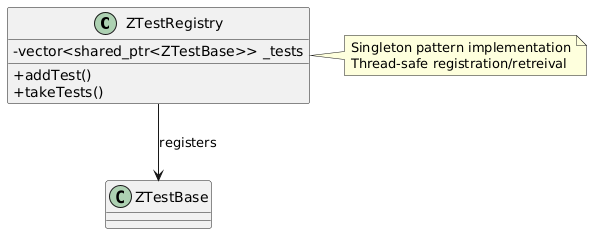
\includegraphics[width = 0.7\textwidth]{img/c2.png} % Assume logo.png is the school logo image file
    \caption{Ztest Class Diagram}
    \label{fig:ztest class }
\end{figure}
\subsubsection{Test Execution Related Classes}
\begin{itemize}
    \item \texttt{ZTestContext} (ztest\_context.hpp): The test execution context uses the Strategy pattern to select execution strategies based on test types and implements parallel test execution with the Thread Pool pattern.
    \item \texttt{ZThreadPool} (ztest\_thread.hpp): A thread pool implementation that uses the Object Pool pattern, manages task queues with the Producer-Consumer pattern, and implements asynchronous execution monitoring with future/promise mechanisms.
\end{itemize}
\begin{figure}[H]
    \centering
    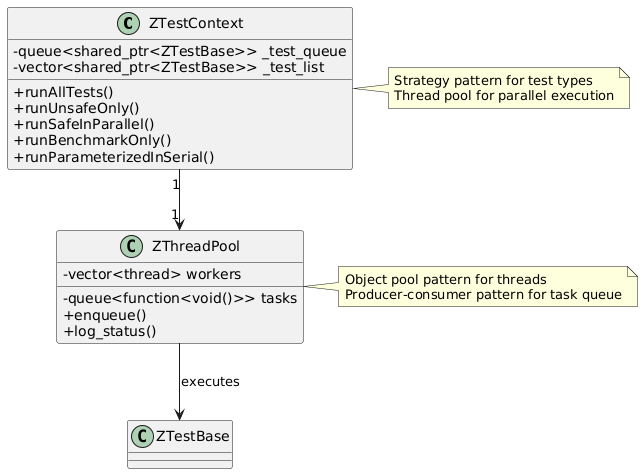
\includegraphics[width = 0.7\textwidth]{img/c3.png} % Assume logo.png is the school logo image file
    \caption{Ztest Class Diagram}
    \label{fig:ztest class }
\end{figure}
\subsubsection{Data Management Related Classes}
\begin{itemize}
    \item \texttt{ZDataRegistry} (ztest\_dataregistry.hpp): A data cache manager implemented with the Singleton pattern for global access, using an LRU strategy for cache eviction.
    \item \texttt{ZDataManager} (ztest\_parameterized.hpp): An abstract base class for data management, providing data management interfaces and implementing iterator-like functionality similar to Python.
    \item \texttt{ZTestDataManager} (ztest\_parameterized.hpp): A generic class that implements test data management functionality for user-specified data types in the code.
    \item \texttt{ZTestCSVDataManager} (ztest\_parameterized.hpp): A class that inherits from \texttt{ZTestDataManager} and \texttt{ZDataManager}, implementing the functionality of reading test data from CSV files and processing it into a form suitable for parameterized testing.
\end{itemize}
\begin{figure}[H]
    \centering
    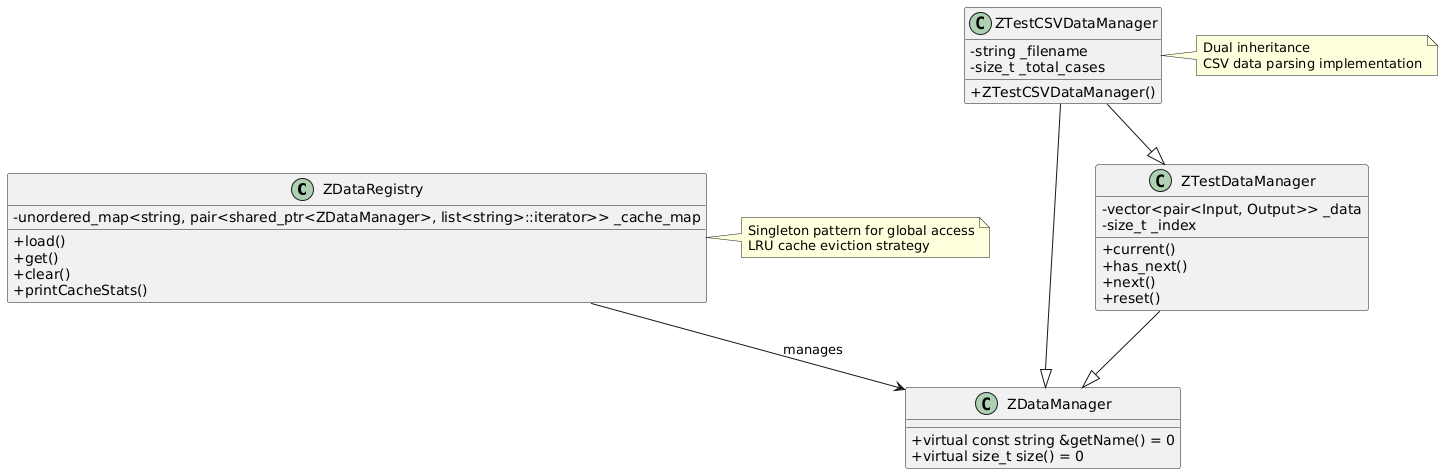
\includegraphics[width = \textwidth]{img/c4.png} % Assume logo.png is the school logo image file
    \caption{Ztest Class Diagram}
    \label{fig:ztest class }
\end{figure}
\subsubsection{Result Management Related Classes}
\begin{itemize}
    \item \texttt{ZTestResult} (ztest\_result.hpp): A test result class implemented with the Value Object pattern, encapsulating immutable data such as test status and duration.
    \item \texttt{ZTestResultManager} (ztest\_result.hpp): A result manager implemented with the Singleton pattern, using the Chain of Responsibility pattern to handle result storage and querying.
\end{itemize}
\begin{figure}[H]
    \centering
    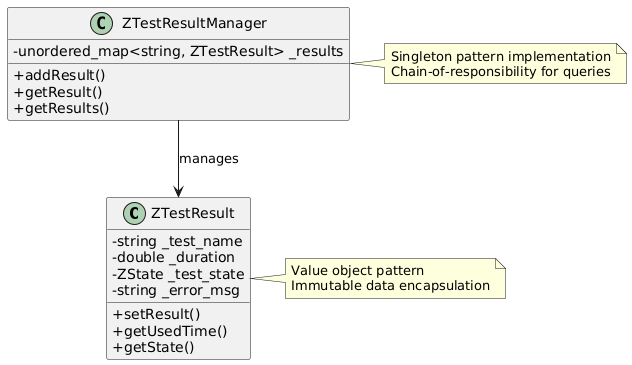
\includegraphics[width = 0.7\textwidth]{img/c5.png} % Assume logo.png is the school logo image file
    \caption{Ztest Class Diagram}
    \label{fig:ztest class }
\end{figure}
\subsubsection{Report Generation Related Classes}
\begin{itemize}
    \item \texttt{ZLogger} (ztest\_logger.hpp): A multi-format report generator that uses the Template Method pattern to define the report generation process and supports HTML, JSON, and JUnit report formats.
\end{itemize}
\begin{figure}[H]
    \centering
    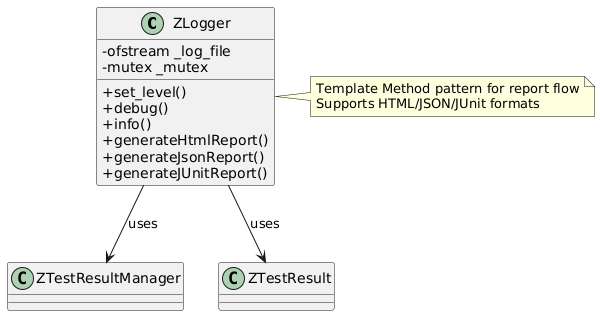
\includegraphics[width =0.7\textwidth]{img/c6.png} % Assume logo.png is the school logo image file
    \caption{Ztest Class Diagram}
    \label{fig:ztest class }
\end{figure}
\subsubsection{Utility Module Related Classes}
\begin{itemize}
    \item \texttt{ZTimer} (ztest\_timer.hpp): A timer implemented with the RAII pattern, encapsulating time measurement functionality.
    \item \texttt{CSVStream} (ztest\_utils.hpp): Implements CSV stream operations similar to the standard input/output library, supporting read, write, and basic information printing.
\end{itemize}
\begin{figure}[H]
    \centering
    \includegraphics[width = \textwidth]{img/c7.png} % Assume logo.png is the school logo image file
    \caption{Ztest Class Diagram}
    \label{fig:ztest class }
\end{figure}
\subsubsection{GUI Module Related Classes}
\begin{itemize}
    \item \texttt{ZTestModel} (gui.hpp): The Model layer in the MVC architecture, using the Observer pattern to monitor test status changes.
    \item \texttt{ZTestController} (gui.hpp): The Controller layer in the MVC architecture, implementing the Command pattern to encapsulate test execution operations.
    \item \texttt{ZTestView} (gui.hpp): The View layer in the MVC architecture, using the Bridge pattern to separate interface elements from implementation.
\end{itemize}
\begin{figure}[H]
    \centering
    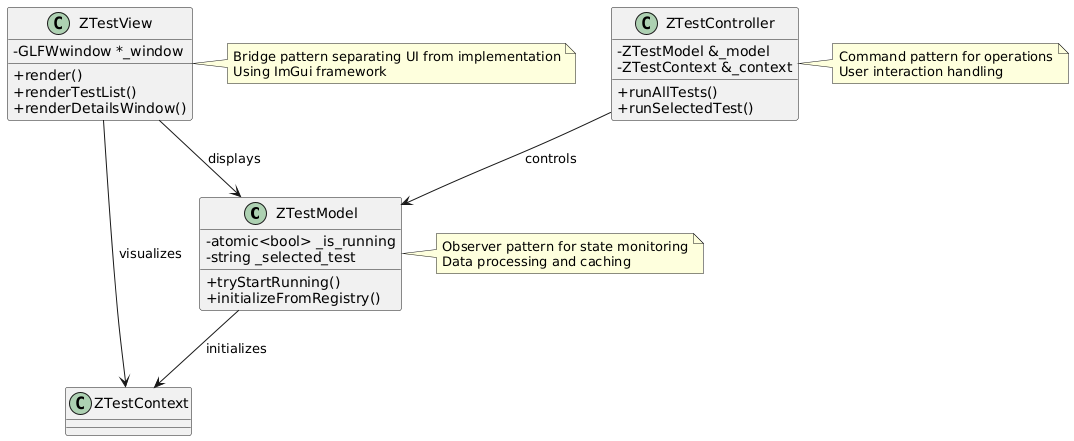
\includegraphics[width = \textwidth]{img/c8.png} % Assume logo.png is the school logo image file
    \caption{Ztest Class Diagram}
    \label{fig:ztest class }
\end{figure}
\section{Programming Progress}
\begin{table}[H]
    \centering
    \begin{tabular}{|m{5cm}|m{2cm}|m{5cm}|m{3cm}|}
        \toprule
        \textbf{Task Phase}                     & \textbf{Time}         & \textbf{Plan}                                                        & \textbf{Actual } \\ \midrule
        \textbf{Determine Topic}                & 2024.04.26-2024.05.03 & Investigate the topic and submit a proposal.                         & Done             \\ \midrule
        \textbf{Implement Core Code}            & 2024.05.03-2024.05.05 & Implemented the execution logic of GUI and Safe test and Unsafe test & Done             \\ \midrule
        \textbf{Major Performance Optimization} & 2024.05.05-2024.05.08 & Thread pool optimization                                             & Done             \\ \midrule
        Function Optimization                   & 2024.05.08-2024.05.11 & Improved JSON, HTML output, JUnit format output, CI integration      & Done             \\ \midrule
        Function Optimization                   & 2024.05.11-2024.05.13 & Introduced imgui Docking functionality in GUI                        & Done             \\ \midrule
        Function Optimization                   & 2024.05.13-2024.05.15 & Added CLI                                                            & Done             \\ \midrule
        \textbf{Major Function Optimization}    & 2024.05.15-2024.05.24 & Added BENCHMARK testing                                              & Done             \\ \midrule
        Function Optimization                   & 2024.05.24-2024.05.25 & Added device status monitoring and visualization                     & Done             \\ \midrule
        \textbf{Major Function Optimization}    & 2024.05.25-2024.05.28 & Added parameterized testing and data-driven functionality            & Done             \\ \midrule
        \textbf{Major Performance Optimization} & 2024.05.28-2024.06.02 & Implemented caching and LRU cache eviction for data                  & Done             \\ \midrule
        \textbf{Major Function Optimization}    & 2024.06.02-2024.06.04 & Added AI diagnosis                                                   & Done             \\ \midrule
        \textbf{Summary Work}                   & 2024.06.04-2024.06.05 & Cross-platform porting \& Report writing                             & Done             \\
        \bottomrule
    \end{tabular}
    \caption{Programming Progress}
\end{table}
\section{Test Report}
\subsection{Functional Testing \& System Testing}
\subsubsection{Assertion Function Testing}
This test aims to verify the behavior of assertion macros such as EXPECT\_EQ, EXPECT\_NEAR, and ASSERT\_TRUE in both successful and failed cases. By designing different test cases, we can check whether these assertions correctly identify the match between expected and actual results, ensuring that the assertion function of the test framework works reliably.
\begin{framed}
    \begin{lstlisting}[language=C++]
int add(int a, int b) { return a + b; }
double subtract(double a, double b) { return a - b; }
ZTEST_F(ASSERTION, FailedEXPECT_EQ) {
  EXPECT_EQ(6, add(2, 3));
  return ZState::z_success;
}
ZTEST_F(ASSERTION, SuccessEXPECT_EQ) {
  EXPECT_EQ(5, add(2, 3));
  return ZState::z_success;
}
ZTEST_F(ASSERTION, SuccessEXPECT_NEAR) {
  EXPECT_NEAR(2, subtract(5.0, 3.0), 0.001);
  return ZState::z_success;
}

ZTEST_F(ASSERTION, FailedEXPECT_NEAR) {
  EXPECT_NEAR(2, subtract(5.1, 3.0), 0.001);
  return ZState::z_success;
}

ZTEST_F(ASSERTION, FailedASSERT_TRUE) {
  ASSERT_TRUE(false);
  return ZState::z_success;
}
ZTEST_F(ASSERTION, SuccessASSERT_TRUE) {
  ASSERT_TRUE(true);
  return ZState::z_success;
}
\end{lstlisting}
\end{framed}
\begin{figure}[H]
    \centering
    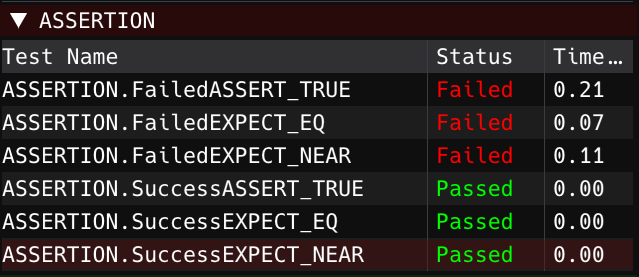
\includegraphics[width=0.7\textwidth]{img/ass.png} % Assume logo.png is the school logo image file
    \caption{Assertion Function Test}
    \label{fig:assertion function test}
\end{figure}
\subsubsection{Test Management Testing}
This test module aims to verify the completeness and reliability of the test management system. By defining various test cases, including single safe tests, single unsafe tests, and test suites with multiple assertions, the system can comprehensively cover different test scenarios. Additionally, the dynamic test case construction functionality allows flexible creation and registration of new test cases, further enhancing the extensibility of the test framework. During testing, memory allocation, function call verification, and assertion checks ensure the correct execution of test cases and consistency with expected results. Moreover, the test framework provides setup and teardown hooks for necessary configurations and cleanup operations before and after tests, ensuring the stability of the test environment and the accuracy of test results.
\begin{framed}
    \begin{lstlisting}[language=C++]
ZTEST_F(TESTMANAGE, safe_test_single_case, safe) {
  ASSERT_TRUE(true);
  return ZState::z_success;
}
ZTEST_F(TESTMANAGE, unsafe_test_single_case, unsafe) {
  ASSERT_TRUE(true);
  return ZState::z_success;
}
ZTEST_F(TESTMANAGE, test_suite) {
  const size_t MB100 = 100 * 1024 * 1024;
  auto ptr = std::make_unique<char[]>(MB100);
  ASSERT_TRUE(ptr != nullptr);
  EXPECT_EQ(3, subtract(5, 3));
  EXPECT_EQ(6, add(2, 3));
  return ZState::z_success;
}
void createSingleTestCase() {
  // Use TestBuilder to construct test
  auto test =
      TestFactory::createTest("AdditionTest",                // Test name
                              ZType::z_safe,                 // Execution
                              "Test addition functionality", // Description
                              add, 2, 3 // Function and arguments
                              )
          .setExpectedOutput(5) // Set expected result
          .beforeAll([]() {     // Setup hook
            std::cout << "Setting up single test..." << std::endl;
          })
          .afterEach([]() { // Teardown hook
            std::cout << "Cleaning up after test..." << std::endl;
          })
          .withDescription("Verify basic addition")
          .registerTest()
          .build(); // Register with test
}
// in main()
createSingleTestCase();

\end{lstlisting}
\end{framed}
\begin{figure}[H]
    \centering
    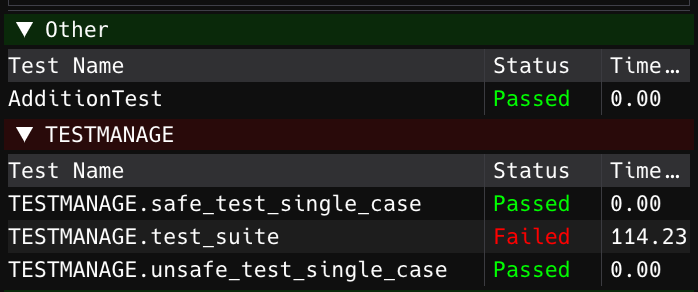
\includegraphics[width=0.7\textwidth]{img/manage.png} % Assume logo.png is the school logo image file
    \caption{Test Management Function Test}
    \label{fig:test management function test}
\end{figure}
\newpage
\subsubsection{Test Execution Management}
In this test module, the efficiency and accuracy of the test execution management mechanism are primarily verified. Multiple safe and unsafe test cases are defined to simulate different execution times and task types. Each test case uses the sleep function to simulate different execution times to test the performance differences between parallel and sequential execution.
The test results are explained as follows:
\begin{itemize}
    \item A thread pool with eight threads is used to execute three test cases in parallel.
    \item Three test cases are executed sequentially.
\end{itemize}
\begin{framed}
    \begin{lstlisting}[language=C++]
ZTEST_F(RUN, safe_test_single_case1, safe) {
  sleep(2);
  ASSERT_TRUE(true);
  return ZState::z_success;
}
ZTEST_F(RUN, safe_test_single_case2, safe) {
  sleep(1);
  ASSERT_TRUE(true);
  return ZState::z_success;
}
ZTEST_F(RUN, safe_test_single_case3, safe) {
  sleep(3);
  ASSERT_TRUE(true);
  return ZState::z_success;
}
ZTEST_F(RUN, unsafe_test_single_case1, unsafe) {
  sleep(1);
  EXPECT_EQ(false, false);
  return ZState::z_success;
}
ZTEST_F(RUN, unsafe_test_single_case2, unsafe) {
  sleep(2);
  EXPECT_EQ(false, false);
  return ZState::z_success;
}
ZTEST_F(RUN, unsafe_test_single_case3, unsafe) {
  sleep(3);
  EXPECT_EQ(false, false);
  return ZState::z_success;
}
\end{lstlisting}
\end{framed}
\begin{figure}[H]
    \centering
    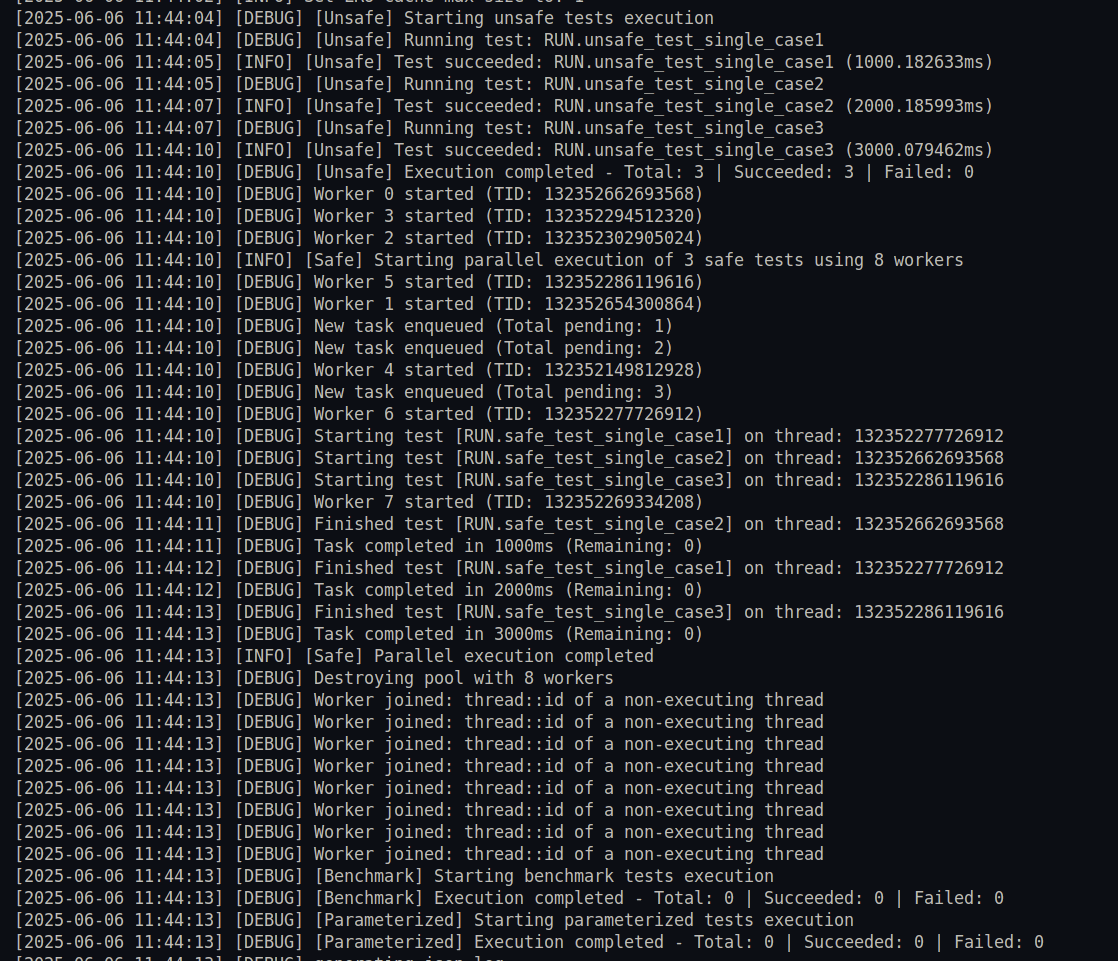
\includegraphics[width=\textwidth]{img/context.png}
    \caption{Test Executor Function Test}
    \label{fig:test executor function test}
\end{figure}

\subsubsection{Data-Driven Testing}
Two types of data-driven test cases are demonstrated, using in-memory datasets and external CSV files as data sources for testing.

\begin{framed}
    \begin{lstlisting}[language=C++]
ZTestDataManager<vector<int>, int> sum_test_data = {
    {{1, 2}, 3}, {{-1, 1}, 0}, {{10, 20}, 30}};
ZTEST_P(ArithmeticSuite, SumTest, sum_test_data) {
  auto &&[inputs, expected] = _data.current();
  int actual = inputs[0] + inputs[1];
  EXPECT_EQ_FOREACH(expected, actual);
  return ZState::z_success;
}
ZTestDataManager<tuple<float, int>, float> sum_test_data2 = {
    {{1.2, 2}, 3.2}, {{-1.0, 1}, 0.0}, {{10.1, 20}, 30.2}};
ZTEST_P(ArithmeticSuite, SumTestfordiff, sum_test_data2) {
  auto &&[inputs, expected] = _data.current();
  float actual = std::get<0>(inputs) + std::get<1>(inputs);
  EXPECT_EQ_FOREACH(expected, actual);
  return ZState::z_success;
}
ZTEST_P_CSV(MathTests, AdditionTests, "data.csv") {
  auto inputs = getInput();
  auto expected = getOutput();
  double actual = std::get<double>(inputs[0]) + std::get<double>(inputs[1]);
  EXPECT_EQ(actual, std::get<double>(expected));
  return ZState::z_success;
}
\end{lstlisting}
\end{framed}
\begin{figure}[H]
    \centering
    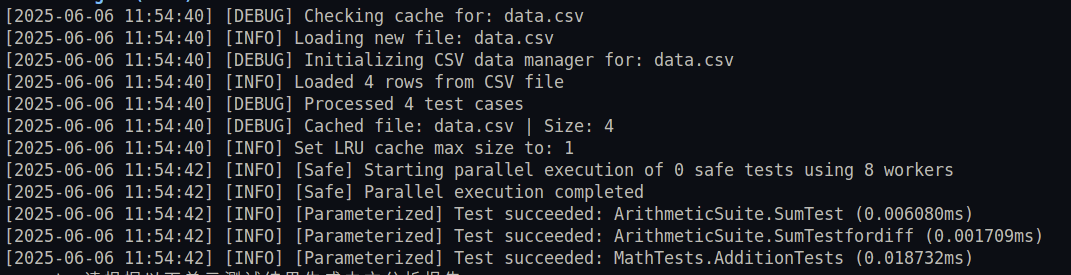
\includegraphics[width=\textwidth]{img/data.png}
    \caption{Data-Driven Function Test}
    \label{fig: Data-Driven Function Test}
\end{figure}
\subsubsection{Benchmark Testing}
Testing the definition of benchmark-type tests, visualization of test time distribution, and monitoring of CPU and memory usage on the GUI.

\begin{framed}

    \begin{lstlisting}[language=C++]
ZBENCHMARK(Vector, PushBack) {
  std::vector<int> v;
  for (int i = 0; i < 10000; ++i)
    v.push_back(i);
  return ZState::z_success;
}
ZBENCHMARK(Matrix, PushBack, 20000) {
  std::vector<int> v;
  for (int i = 0; i < 1000; ++i)
    v.push_back(random());
  return ZState::z_success;
}\end{lstlisting}
\end{framed}
\begin{figure}[H]
    \centering
    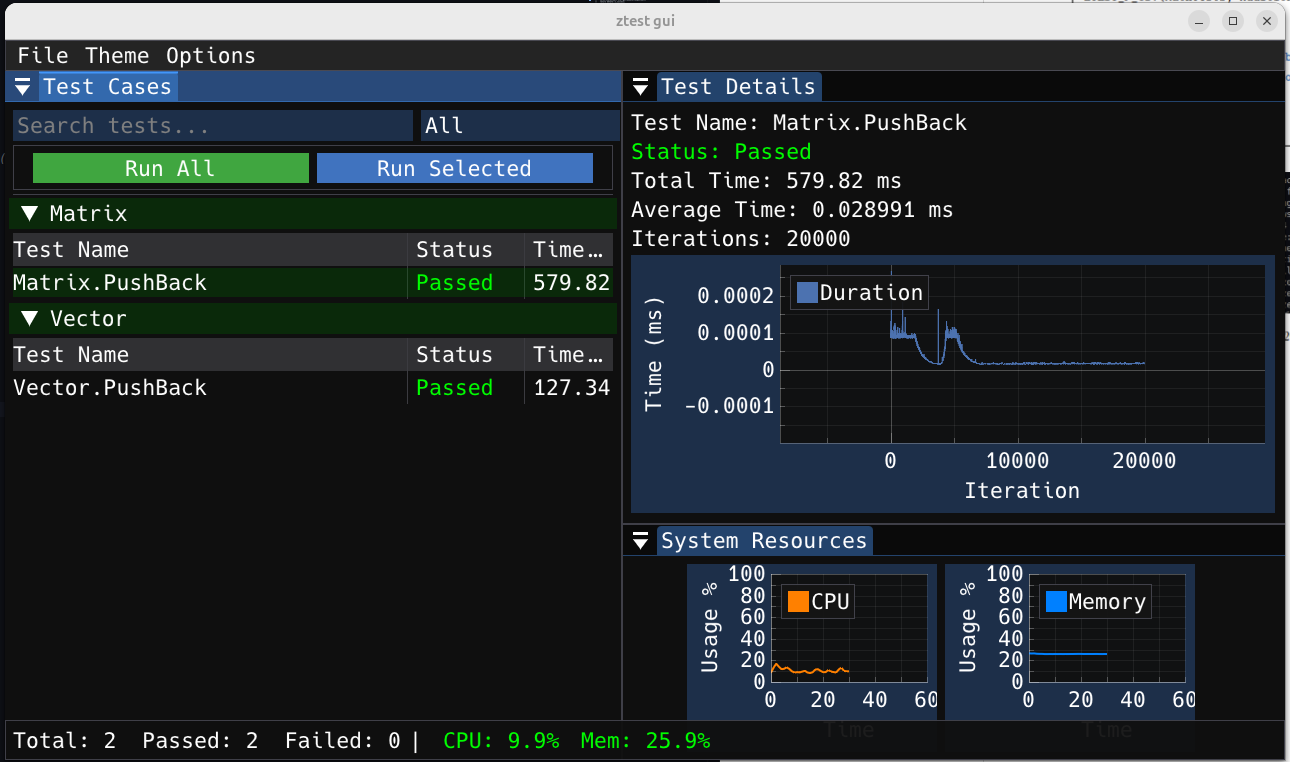
\includegraphics[width=\textwidth]{img/ben.png}
    \caption{Benchmark Function Test}
    \label{fig: Benchmark Function Test}
\end{figure}

\begin{itemize}
    \item
\end{itemize}
\subsubsection{Report Generation Testing}

Testing the generation of HTML, JSON, and XML format reports.
\begin{figure}[H]
    \centering
    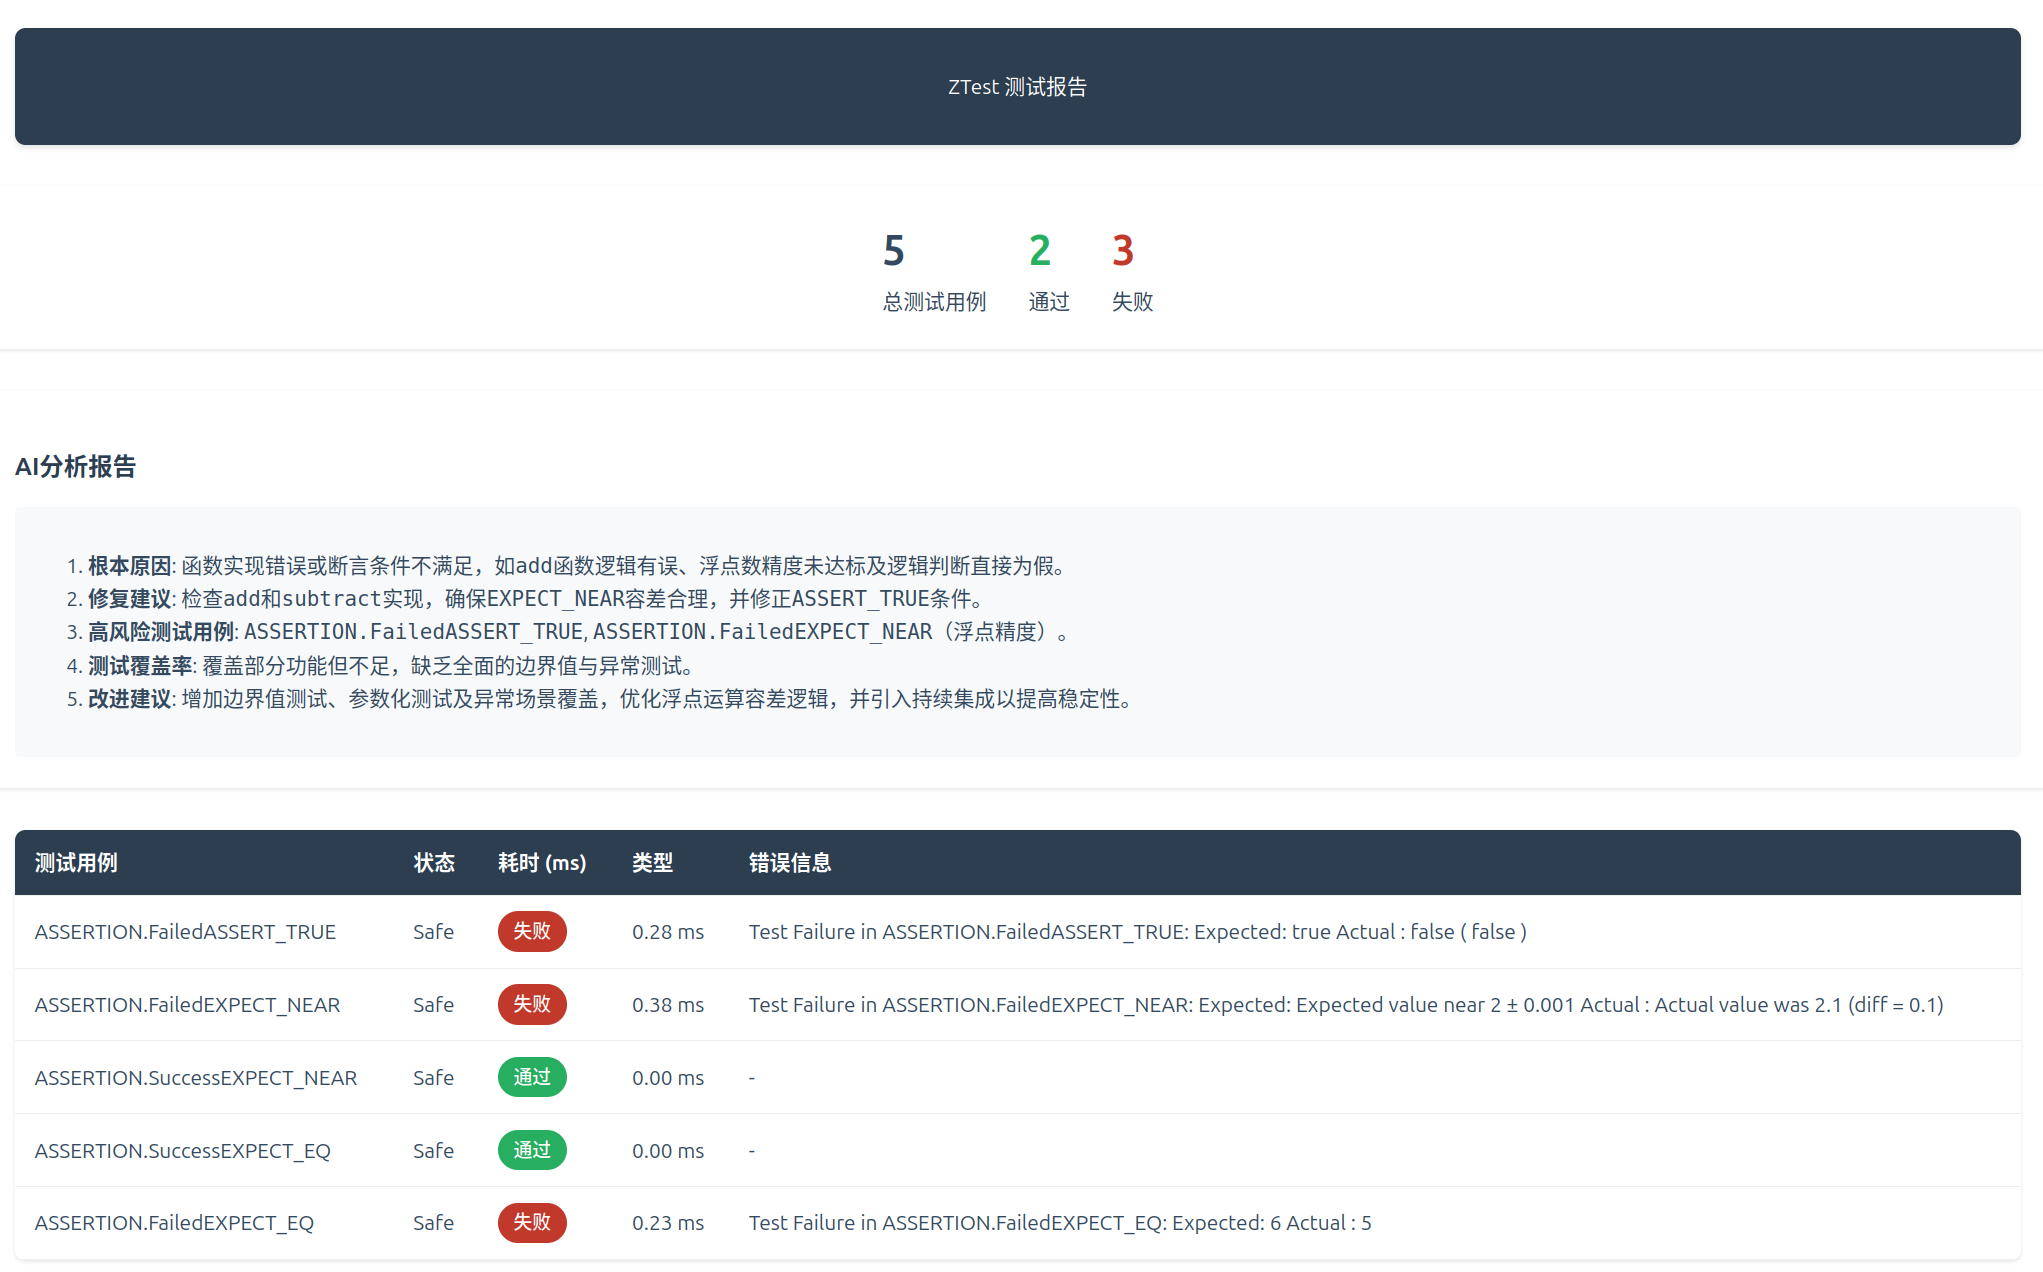
\includegraphics[width=0.8\textwidth]{img/html.png}
    \caption{HTML Test Report}
    \label{fig: HTML Test Report}
\end{figure}
\begin{figure}[H]
    \centering
    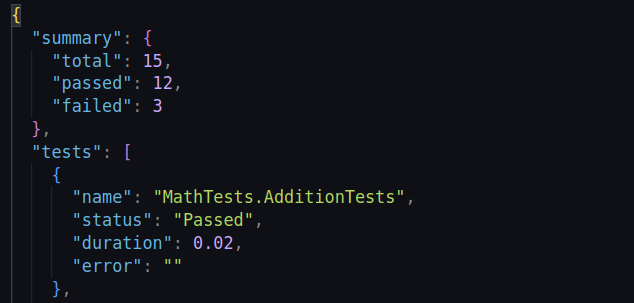
\includegraphics[width=0.6\textwidth]{img/json.png}
    \caption{Partial JSON Report}
    \label{fig: Partial JSON Report}
\end{figure}

\begin{figure}[H]
    \centering
    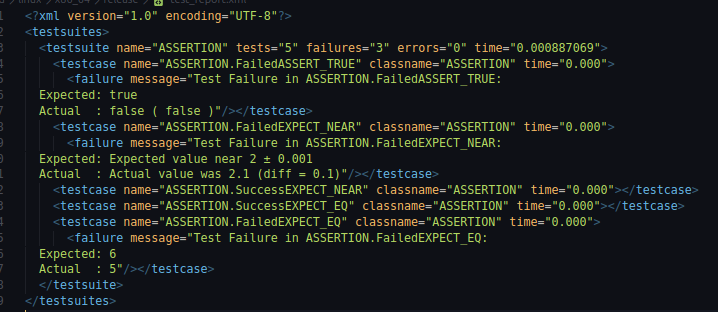
\includegraphics[width=0.6\textwidth]{img/xml.png}
    \caption{XML (JUnit Format) Report}
    \label{fig: XML (JUnit Format) Report}
\end{figure}
\subsubsection{GUI Testing}
Testing the display of the GUI, theme switching, AI assistant display, and other functions.
\begin{figure}[H]
    \centering
    \begin{minipage}{0.5\textwidth}
        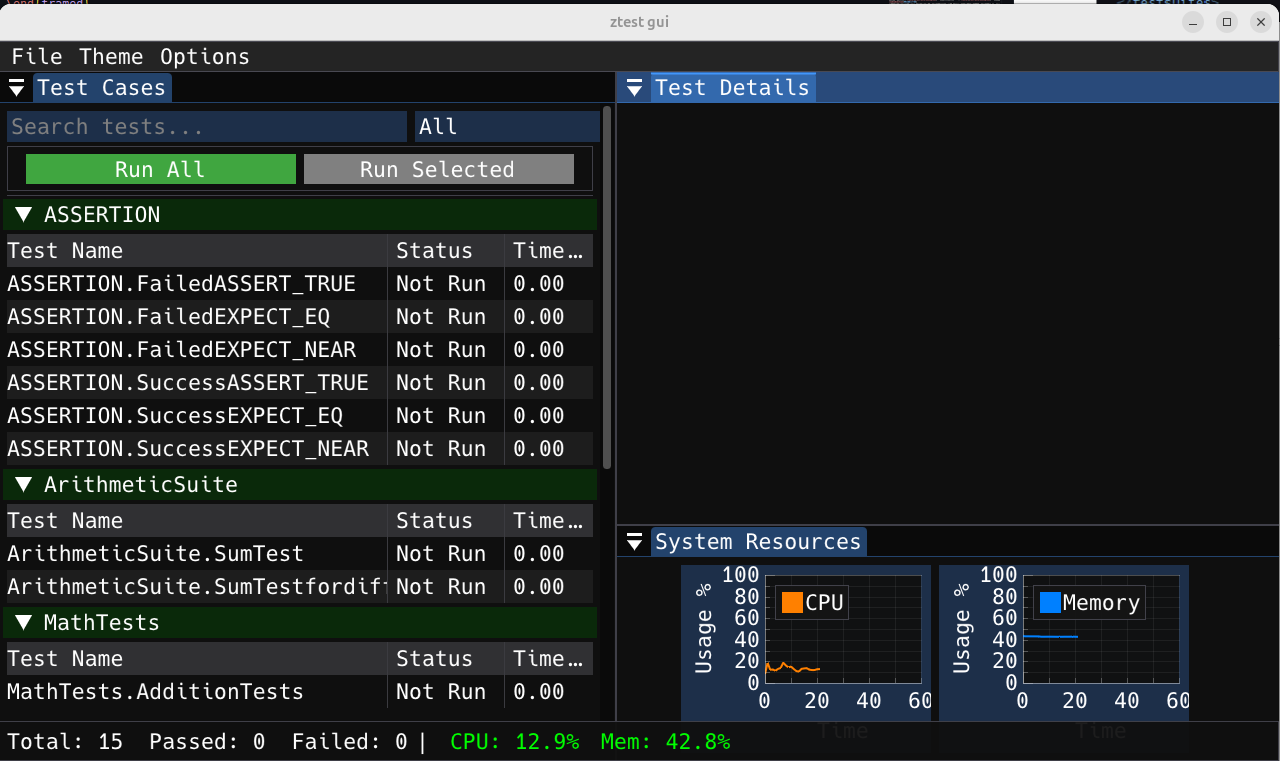
\includegraphics[width=\textwidth]{img/showgui.png}
        \caption{Dark Theme GUI Display}
        \label{fig:showgui}
    \end{minipage}%
    \begin{minipage}{0.5\textwidth}
        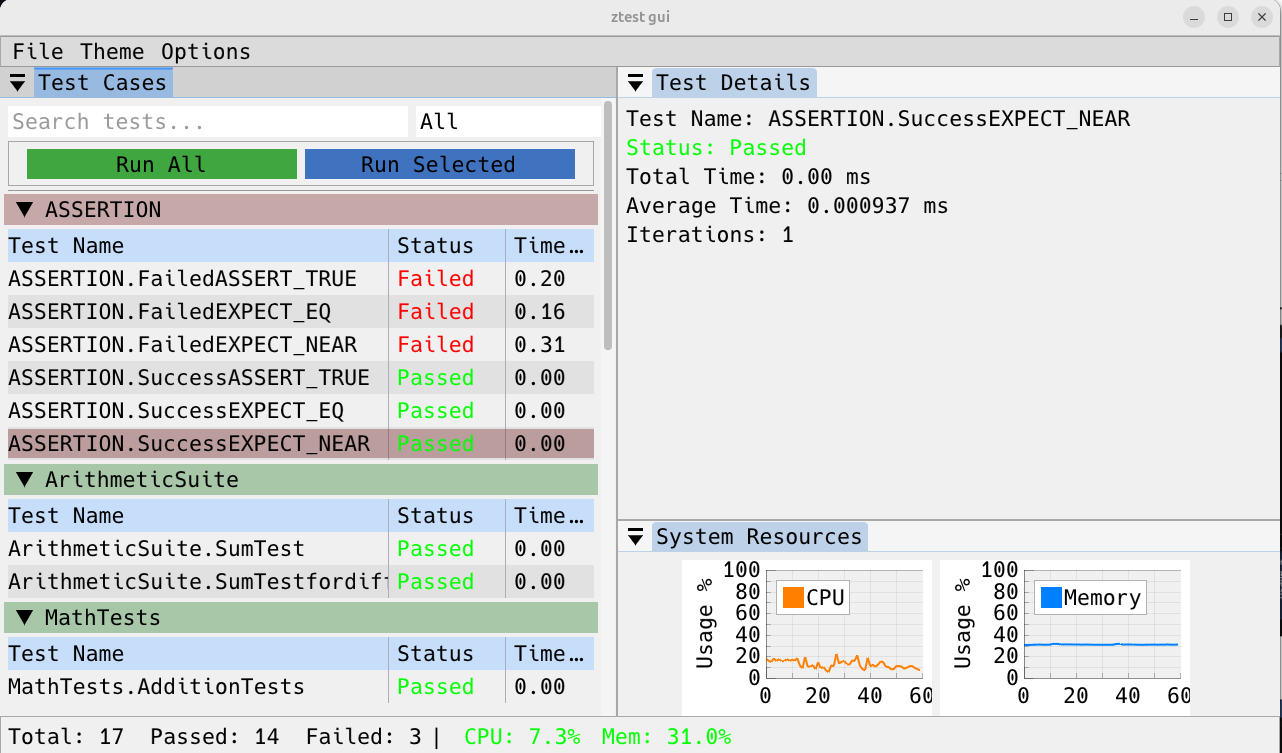
\includegraphics[width=\textwidth]{img/light.png}
        \caption{Light Theme GUI Display}
        \label{fig:light}
    \end{minipage}
\end{figure}
\begin{figure}[H]
    \centering
    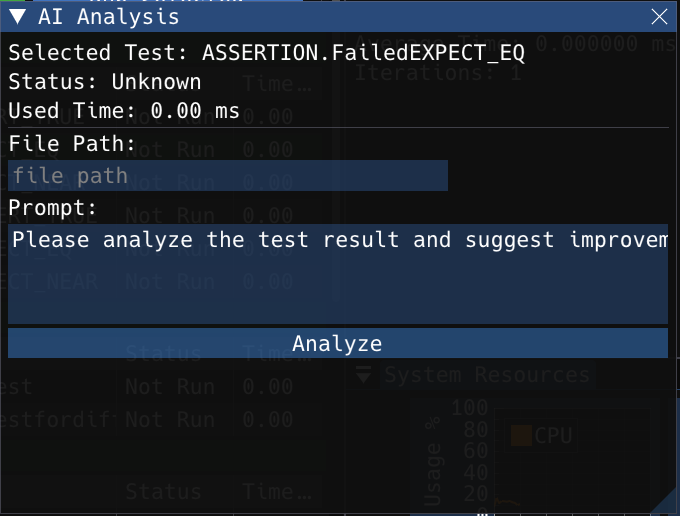
\includegraphics[width=0.4\textwidth]{img/aih.png}
    \caption{AI Diagnosis Assistant Display}
    \label{fig: AI Diagnosis Assistant Display}
\end{figure}
\subsubsection{AI Diagnosis Testing}
When generating reports, AI (qwen turbo) is called for diagnosis and written into the HTML report.
\begin{figure}[H]
    \centering
    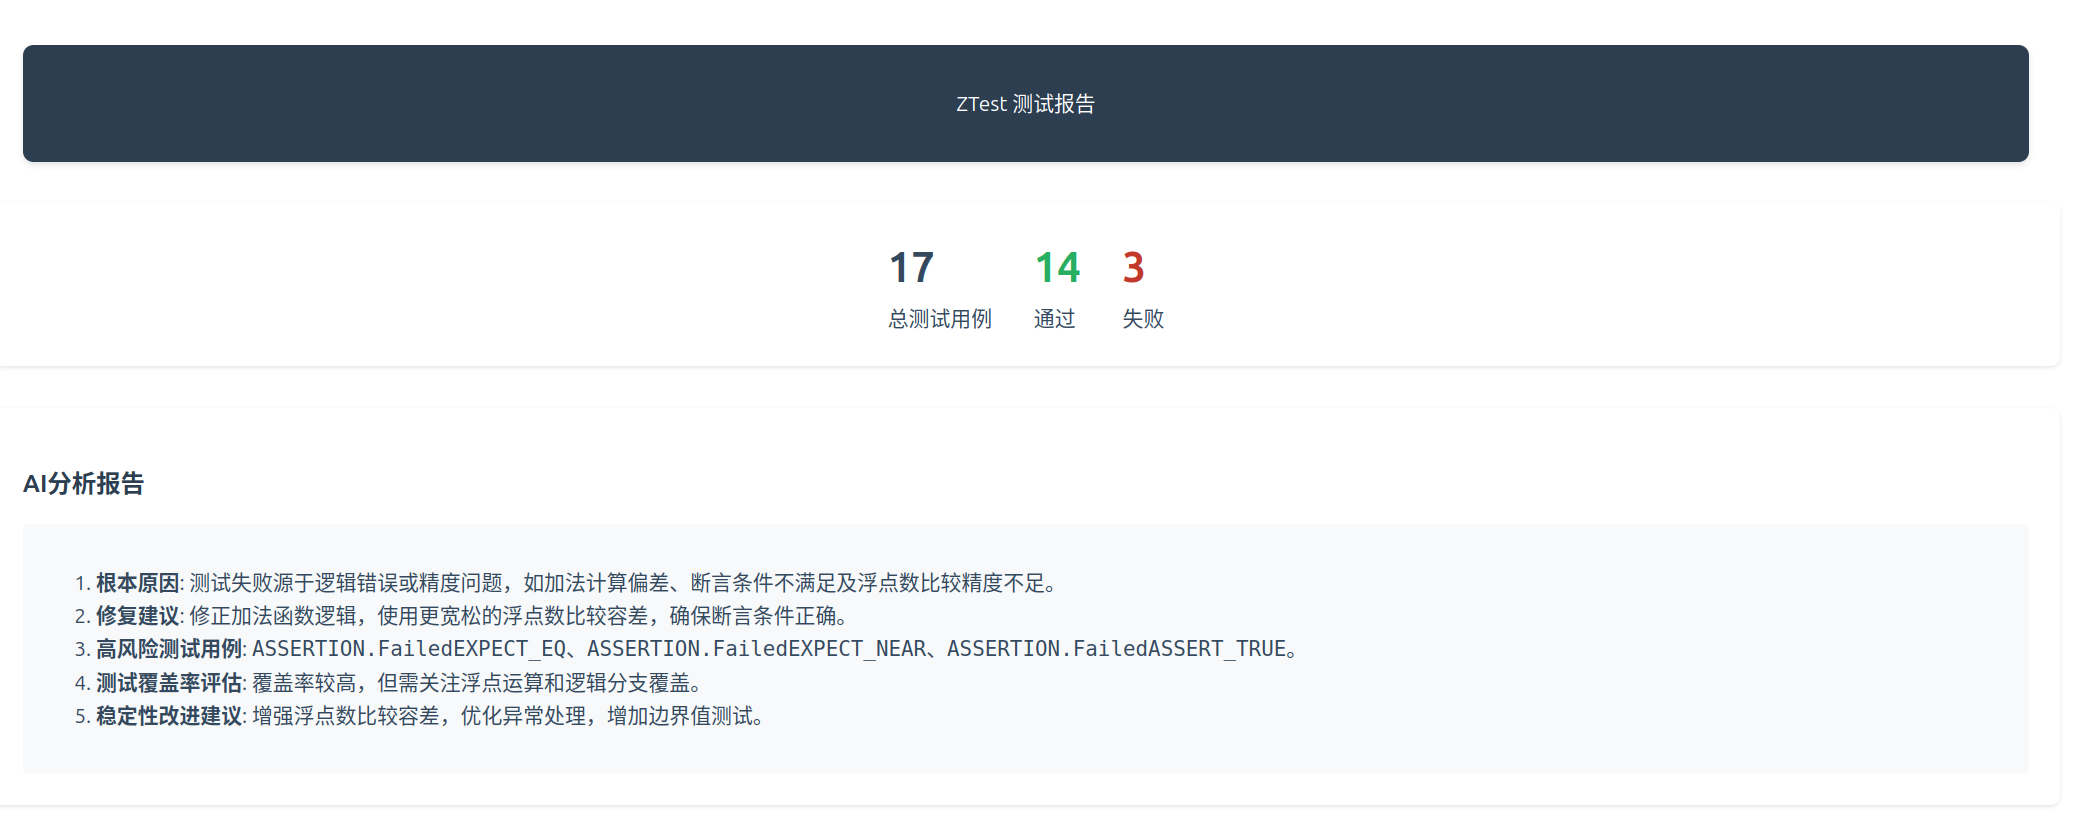
\includegraphics[width=\textwidth]{img/ai.png}
\end{figure}
In the GUI interface, AI (qwen turbo) is called for diagnosis of individual test cases and displayed, allowing users to input custom prompts and file paths for the test.
\begin{figure}[H]
    \centering
    \begin{minipage}{0.45\textwidth}
        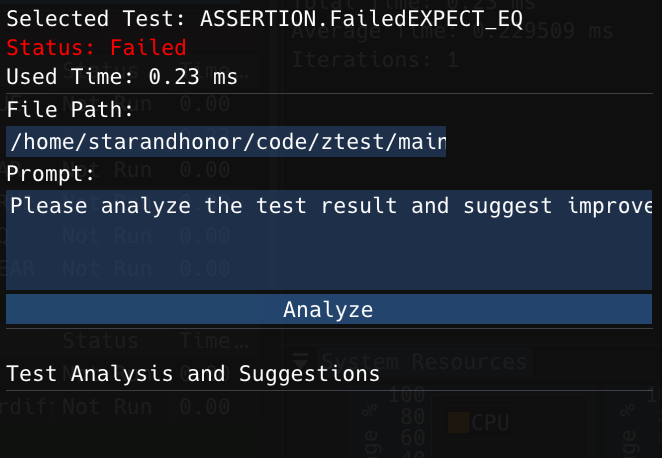
\includegraphics[width=\textwidth]{img/aih1.png}
    \end{minipage}
    \hfill
    \begin{minipage}{0.45\textwidth}
        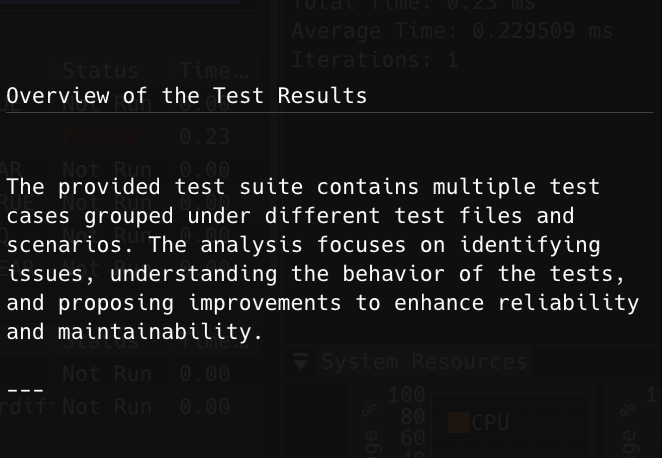
\includegraphics[width=\textwidth]{img/aih2.png}
    \end{minipage}
\end{figure}


\section{Personal Summary}
\begin{tabular}{|p{50pt}|p{350pt}|}
    \hline
    Name           & Insights                                                                                                                                                                                                                                                                                                                                                                                                                                                                                                                                                                                                 \\ \hline
    Zheng Chenyang & Emphasized the importance of modular design and layered architecture. By introducing the MVC pattern, the maintainability and scalability of the code were enhanced. Optimized resource monitoring and task scheduling in a multi-threaded environment to ensure system stability and performance. Combined AI analysis capabilities to provide intelligent feedback on test results, enhancing the tool's practicality. Future work will continue to iterate and improve functionality and user experience.                                                                                             \\ \hline
    Ye Suohua      & Mainly responsible for interface development, using the imgui library to complete the front-end architecture and rendering. Realized that front-end design needs to be based on user requirements, considering cross-platform compatibility and library version issues.                                                                                                                                                                                                                                                                                                                                  \\ \hline
    Qi Yansong     & Participated in the development of the "ztest" unit testing framework, applying it to game development and tool software design. Through innovative design, addressed the shortcomings of existing frameworks (such as Google Test) in GUI support, concurrent testing, and reporting systems, improving user experience and scalability. Through practice, gained a deeper understanding of modern C++ features and design patterns, recognizing that excellent software products need to balance technical depth and user experience, and that efficient team communication and collaboration are key. \\ \hline
    Wang Ruizhen   & Faced challenges in this large-scale complex project, practiced and learned new knowledge and skills, and enhanced problem-solving abilities.                                                                                                                                                                                                                                                                                                                                                                                                                                                            \\ \hline
    Wu Hongqing    & Responsible for the GUI design of the ztest project, using the ImGui framework to implement a visual interface. Designed simple and intuitive windows, coordinated the ZTestModel, ZTestView, and ZTestController classes, and improved user-friendliness. Through team collaboration, enhanced team cooperation skills and reduced compilation errors and understanding difficulties.                                                                                                                                                                                                                   \\ \hline
\end{tabular}
\section{References}
\begin{thebibliography}{99}
    \bibitem{gtest} Google Test. \textit{Google Test Documentation}. [Online]. Available: https://github.com/google/googletest
    \bibitem{junit} JUnit. \textit{JUnit Documentation}. [Online]. Available: https://junit.org/junit5/
    \bibitem{catch} Catch2. \textit{Catch2 Documentation}. [Online]. Available: https://github.com/catchorg/Catch2
    \bibitem{gtest-parallel} Google Test Parallel. \textit{Google Test Parallel Documentation}. [Online]. Available: https://github.com/google/gtest-parallel
    \bibitem{pytest} Pytest. \textit{Pytest Documentation}. [Online]. Available: https://docs.pytest.org/en/latest/
    \bibitem{miniunit} MiniUnit. \textit{MiniUnit Documentation}. [Online]. Available: https://github.com/urin/miniunit
\end{thebibliography}

\end{document}